\documentclass[12pt,a4paper,english
% ,twoside,openright
]{tunithesis}

% Note that you must choose either Finnish or English here and there in this
% file.
% Other options for document class
  % ,twoside,openright   % If printing on both sides (>80 pages)
  % ,twocolumn           % Can be used in lab reports, not in theses

% Ensure the correct Pdf size (not needed in all environments)
\special{papersize=210mm,297mm}


% LaTeX file for BSC/MSc theses and lab reports.
% Requires the class file (=template) tunithesis.cls and figure files,
% either tut-logo, exampleFig (as pdf or eps) and example_code.c
% Author: Lucas Machado (2018)
% Based on TTU template by Sami Paavilainen (2006), modified by Heikki Huttunen (2014)


% More information about Latex basics:
% [Tobias Oetiker, Hubert Partl, Irene Hyna, Elisabeth Schlegl, The
% Not So Short Introduction to LATEX2e, Version 5.03, April 2014, 171
% pages.  Availbale: http://tobi.oetiker.ch/lshort/lshort.pdf]


%
% Define your basic information
%
\author{Chen Zhu}
\title{Machine Learning Approach of Logistic Organ Dysfunction Score Prediction with Data Acquired from Bedside in ICU} % primary title (for front page)
\thesistype{Master's thesis} % or Bachelor of Science, Laboratory Report... 

% Put your thesis' main language last
% http://mirrors.ctan.org/macros/latex/required/babel/base/babel.pdf
\usepackage{lastpage}
\usepackage{comment}
\usepackage{multirow}
\usepackage[english]{babel}
\usepackage[
backend=biber,
style=authoryear,
citestyle=authoryear,
autocite=inline
]{biblatex}
\usepackage{csquotes}
\usepackage{lscape} 
\usepackage{threeparttable}
\usepackage{amsfonts}



\addbibresource{thesis_refs.bib} %Imports bibliography file

%
% You can include special packages or define new commands here at the
% beginning. Options are given in brackets and package name is in
% braces:  \usepackage{opt]{pkg_name}

% Option1) for bibliography does not need additional packages.

% Option2b) for bibliography: old way for using Name-year citations
% http://www.ctan.org/tex-archive/macros/latex/contrib/harvard/ 
%\usepackage{harvard}  


% Option3) for bibliography: newer way, esp. for Name-year citations
% http://www.ctan.org/pkg/biblatex
%\usepackage[style=authoryear,maxcitenames=2,backend=bibtex,
%  firstinits=true]{biblatex}
%% Note that option style=numeric works as well
%\addbibresource{thesis_refs.bib}

\definecolor{tunipurple}{RGB}{78, 0, 142}

% You can also add your own commands
\newcommand\todo[1]{{\color{red}!!!TODO: #1}} % Remark text in braces appears in red
\newcommand{\angs}{\textsl{\AA}}              % , e.g. slanted symbol for Ångstöm
%\renewcommand{\thetable}{\arabic{table}}
% Preparatory content ends here



\pagenumbering{roman} % was: {Roman}
\pagestyle{headings}
\begin{document}



% Special trick so that internal macros (denoted with @ in their name)
% can be used outside the cls file (e.g. \@author)
\makeatletter



%
% Create the title page.
% First the logo. Check its language.
\thispagestyle{empty}
\vspace*{-.5cm}\noindent

\begin{figure}
    \vspace{-1.3cm}
    \advance\leftskip-2.5cm
    \noindent
\includegraphics{img/tunilogo.png}
\end{figure}
 
\vspace{2.5cm}
\begin{flushright}
\noindent\textsf{\LARGE{\@author}}

\noindent\vspace{0.5cm}

\noindent\Huge{\textsf{\textbf{\textcolor{tunipurple}{\@title}}}}
\end{flushright}
\vspace{10.7cm} % adjust to 12.7 this if thesis title needs two lines

% Last some additional info to the bottom-right corner
\begin{flushright}  
    \begin{spacing}{1.0}
      \textsf{Faculty of Information Technology and Communication Sciences (ITC)\\
      \@thesistype\\
      April 2024}
    \end{spacing}
\end{flushright}

% Leave the backside of title page empty in twoside mode
\if@twoside
\clearpage
\fi

% Turn off page numbering for the first pages
\pagenumbering{gobble}


% Some fields in abstract are automated, namely those with \@ (author,
% title, thesis type).

\chapter*{Abstract}

\begin{spacing}{1.0}
\noindent \@author: \@title\\
\@thesistype\\
Tampere University\\
Master’s Degree Programme in Software Development\\
April 2024
\end{spacing}
\noindent\rule{12cm}{0.4pt}

\vspace{0.5cm}

% ---------------------------------------
% Abstract and keywords
% ---------------------------------------

\noindent Intensive Care Unit (ICU) is a high-stakes environment in hospitals, where patients are at a higher risk than in other departments, such as organ dysfunction, and are monitored with devices, along with more care workers. Effectively predicting patient status in an ICU is a critical task serving patient health and resource allocation. Logistic Organ Dysfunction Score (LODS), calculated with weighted variables of the worst values in the first 24 hours, is an organ dysfunction scoring system that reflects the severity level of organ systems, and can be converted to the probability of mortality in a certain period. However, LODS calculation requires some laboratory results, such as bilirubin, which costs time and money. Effective prediction of LODS value could measure the patient's overall organ dysfunction situation and calculate the probability of mortality for the patient, providing doctors with assistance in adjusting treatment. Machine learning can utilize large amounts of data and existing algorithms to train effective models for highly accurate prediction tasks.

\noindent There are some studies on predicting organ dysfunction with bedside data and some Electronic Health Records (EHR) information, including demographic information and laboratory results. This thesis proposes machine learning models, trained with the Medical Information Mart for Intensive Care (MIMIC) -IV database, to predict total LODS with data that can be acquired bedside in the first 12 hours of ICU stay, to save time and assist doctors in treatment. The model with the best performance utilized eight features and was trained using XGBoost. It achieved a mean absolute error (MAE) of 1.4173 and a root mean square error (RMSE) of 1.8222. These models enhance the practicality and ease of application of LODS, while providing evidence-supported calculated probabilities of mortality. Moreover, this study fills the gap of predicting LODS.




~

\noindent\textbf{Keywords:} machine learning, organ dysfunction score, bedside data, deep learning

~

\noindent The originality of this thesis has been checked using the Turnitin Originality Check service.


% Add the table of contents


\setcounter{tocdepth}{3}              % How many header level are included
\tableofcontents                      % Create TOC


% The actual text begins here and page numbering changes to 1,2...
% Leave the backside of title empty in twoside mode
\if@twoside
%\newpage
\cleardoublepage
\fi


\renewcommand{\chaptername}{} % This disables the prefix 'Chapter' or
                              % 'Luku' in page headers (in 'twoside'
                              % mode)


\chapter{Introduction}
\label{ch:intro} 

\pagenumbering{arabic}
\setcounter{page}{1} % Start numbering from zero because command
                     % 'chapter*' does page break
                     
% \label{...} allows cross-referencing, e.g. 'as explained in
% Chapter~\ref{ch:intro}' Note that you may have to run the command
% 'latex' or 'pdflatex' twice to get cross-references correctly.  You
% can add labels e.g. to chapters, sections, figures, tables, and
% equations.

% You can write everything into single tex file. Alternatively, you
% can write each chapter into separate file and then include them her
% \include{intro} % no postfix .tex to the command
% \include{related_works} % and so on...

An intensive care unit is defined as an organized system to treat critically ill patients with intensive, targeted, and specialized medical and nursing care. It is equipped with monitoring capabilities, and various methods of physiologic organ support to sustain life in cases that patients have acute organ system insufficiency. Scoring system is one of the tools used in critical care to enable the objective quantification of patient severity, risk stratify patients for clinical prognostication and in research as study inclusion criteria and to demonstrate equivalence of patient groups. \parencite{Marshell2017}

\section{ICU and Scoring System}
Since the first intensive care unit (ICU) was established in Denmark in 1953, the ICU has become a critical element in hospital-care based health care. An ICU's activities are not limited to the geographic area in a hospital, but extend to include emergency department , hospital ward and follow-up clinic \parencite{Marshell2017}. Patients with critical illness might be found throughout a hospital, however, many of them are treated in ICU. ICU mortality varies by different conditions, for instance, according to \textcite{Adhikari2010}, 8-18\% in unselected patients in North America, Europe, Australia, and New Zealand, 35–45\% in heterogeneous cohorts of patients with acute lung injury, and 50–60\% in patients with septic shock. Patients in ICU are in three main categories: those with acute organ dysfunction (including those who receive long-term intensive organ support because of their unclear ultimate outcome), those who had a major procedure and are monitored in the peri-intervention period, and those who are receiving end-of-life care. To give sufficient but not excessive treatment, ICU is divided into different levels. A level 1 ICU provides oxygen, noninvasive monitoring, and intensive nursing care compared to a normal ward, where a level 2 ICU is equipped to deliver invasive monitoring and basic life support for a short period. A level 3 ICU functions as a regional hub for critically ill patients by providing a full spectrum of monitoring and advanced life support technologies. It may be involved in developing the specialty of intensive care through research and education \parencite{Marshell2017}. Patients, families and care providers concern about recovery likelihood, however, prognostication can be difficult in ICU \parencite{Tiffany21}.

%Scoring systems are used to objectively quantify condition severity and risk stratify patients for prognostication in clinical. They are also used as standard tools in critical care research to demonstrate equivalence of patients group \parencite{Tiffany21}. It can broadly be divided into those that are specific for a disease or an organ, for example the Glasgow Coma Scale, and those that are for all ICU patients. The scores that are generic for all ICU patients are broadly divided into: 1) scores that assess severity on admission and predict outcome, for example, Acute Physiology and Chronic Health Evaluation (APACHE), 2) scores that assess the severity of organ dysfunction, for example, Sequential Organ Failure Assessment (SOFA), 3) scores that assess nursing workload using, for example, Nine Equivalents of Nursing Manpower Use Score (NEMS) \parencite{Tiffany21, Jonathan2008, Rapsang2014, Vincent2010}. 
Scoring systems used in ICU usually evaluate mortality risk without clinical status, such as the Simplified Acute Physiology Score (SAPS) \parencite{Gall1984}, and tend to evaluate organ deterioration, such as Multiple Organ Dysfunction Score (MODS) \parencite{Marshall1995}. Calculating these scores gives a quantified condition of patients' organ condition and risk level. Logistic Organ Dysfunction Score (LODS) \parencite{legall96}, as somewhere between mortality prediction score and organ dysfunction score, is developed to assess and characterize the current degree of organ dysfunction \parencite{Tiffany21, Vincent2010}. It selects 12 variables to represent the function of six organ systems, which include laboratory results and non-invasive parameters. This score ranges from 0 to 22 where 0 is no dysfunction and 22 is maximum dysfunction. LODS also includes a logistic regression equation that can convert the score into a probability of in-hospital mortality. Although it was not initially validated for repeated use in ICU, \textcite{Timsit2002} validated that LODS characterized the progression of organ dysfunction accurately in the first 7 days of ICU stay.

\section{Machine Learning}
Machine learning is a subset of artificial intelligence, broadly defined as a machine's ability to replicate human learning processes. It is the foundation behind predictive text, language translation apps, and the way social media feeds are presented \parencite{sara2021}. Quoted to \textcite{samuel1959}, machine learning enables computers to learn and improve from experience without being explicitly programmed. What this means is that a computer program learns with observed data and a learning algorithm to perform a task, such as predicting result. %Generally, data in machine learning is split to two groups, a training set and a test set. As the name suggests, the training set is used to train algorithm where features are included. The test set is used to algorithm performance and it is new to the algorithm. Once an algorithm passes the training and test phases with an acceptable performance, it will be implemented to real world. 
The adoption of machine learning can be found in science, commerce and technology, including the diagnosis of faults in complex systems and consumer services \parencite{jorden2015}. In healthcare, machine learning has evolved for years. It is capable of assisting case triage, enhancing image scanning and segmentation, and supporting decision-making, and it has changed and will shift healthcare epidemiology, for instance, predicting the risk of Nosocomial Clostridium difficile Infection (CDI) and predicting clinical outcomes in Ebola Virus Disease (EVD) Infection using initial clinical symptoms \parencite{Jenna2017, Habehh2021}. In addition, machine learning is applied a lot in electronic health records such as analys heart failure survival \parencite{Panahiazar2015}, medical imaging such as detecting diabetic retinopathy from retinal photographs \parencite{Gulshan2016}, and genetic engineering such as predicting the immunogenic landscape of SARS-CoV-2 \parencite{Malone2020} . With the development of deep learning and explainable AI, machine learning is more widely applied in healthcare.

Machine learning offers greater predictive accuracy than traditional statistics when the knowledge of the source data and problem is not clear, because its algorithms are designed to optimize precision and performance. Leveraging advanced techniques such as distributed computing and parallel processing, machine learning algorithms exhibit superior scalability compared to statistics. Furthermore, machine learning excels in managing vast and intricate datasets, whereas statistics is better suited for analyzing simpler datasets characterized by straightforward relationships between variables.  \parencite{Bzdok2018, Rajula2020}

\section{Motivation and Objectives}
In this study, I aim to bring machine learning to accurately predicting LODS value with bedside data in a first 12 hours of ICU stay. There are motivations:
\begin{itemize}
\item LODS is a hybrid organ dysfunction score. Predicting it will indirectly predict the probability of mortality which will give doctors assistance in adjusting treatment.
\item LODS is already widely used in hospitals in the past 20 years so that doctors are familiar with it. Compared to a new organ dysfunction prediction and probability of mortality prediction from a model, LODS prediction is easier to understand and start to use in clinical.
\item To calculate LODS, both bedside data and laboratory results are needed, which costs money and time. Predicting with data that can be collected from bedside, vital signs and data from bedside monitors, will save money and time.
\end{itemize}
Thus, in this study, I try to use vital signs, data from bedside monitors and other data that can be easily obtained to train models. And I try to reduce the amount of data that are collected directly by care workers, such as the Glasgow Coma Scale \parencite{Jain2023}. The easier the data are collected in a non-invasive approach, the easier the model will be used in clinical. Moreover, LODS is calculated with measurements in the first 24 hours of ICU stay. I try to use data in a shorter time range, the first 12 hours, so that the prediction can support doctors' treatment change earlier than normal in clinical, and may indirectly shorten patients' ICU stay length. 
Numerous studies focus on predicting the probability of mortality with machine learning, but many of them rely on directly using health information, which often lacks supporting evidence. And there are very few studies on predicting LODS, so I want to fill this gap. With the scalability of machine learning, I hope that the methods and conclusions in this study can be applied to predictions of other scoring systems or other data sources.

%Medical score system needs accuracy to reflect patients’ condition, and ease of use to reduce clinician time in using and learning. Only if a score system is substantially better than another one, proved by a large number of research, it will be used in practice. So improving an existed score system is more feasible than replacing, and change should be small but useful. LODS estimates with the worst value of the first 24 hours of ICU stay, both bedside and laboratory measurements, which cost money and time. This research would use only bedside data because they are easy to access, without long-time waiting or money cost. And for some dangerous patients, 24 hours is a long time to collect data. If 24h severity can be predicted early, doctors will be able to change the treatment. LODS is a hybrid scoring system which makes it a good tool in this prediction. As human physiology comprises a complex system, using mathematical models to analyse organ dysfunction may describe systemic host response to infection or injury \parencite{seely2011}. So in this research, machine learning is brought to bedside to predict patients' severity by predicting LODS. ICU has many monitoring devices and produces a large amount lab test results which is a great resource for machine learning model training and research.

%XGBoost algorithm is used for predicting part in this study, supported by \textcite{xgboost_lib}. Convolutional Neural Network is used for feature engineering in some models, supported by TensorFlow library. Some vitals signs, include heart rate, respiratory rate, Systolic blood pressure(sbp), Diastolic blood pressure (dbp), mean arterial pressure (MAP), Oxygen Saturation (SPO2), and temperature in the first 12 hours of ICU stay, and other bed side data, include GCS, GCS eye, GCS motor,the total urine output in the first 12 hours, and the most mechanical ventilation method are taken as input to the models, and output is the total LODS value in the first 24h ICU stay. The target is to check if predicting total LODS value to represent patient's 24h situation with 12h bed side data is possible and practicable.

Two experiments were executed in this study. In Experiment I, I trained two models with XGBoost and variables selected with Pearson Correlation Coefficient and Spearman Correlation Coefficient separately. In Experiment II, I trained models with Convolutional Neural Network and XGBoost combination. All data used in this study comes from the Medical Information Mart for Intensive Care (MIMIC) -IV database.

This document is structured as follow. 
\begin{itemize}
\item Chapter ~\ref{ch:background} provides an overview of basic organ dysfunction scoring systems and fundamental machine learning concepts.
\item Chapter ~\ref{ch:priorwork} reviews prior research conducted in similar fields, focusing primarily on predicting and evaluating patients' conditions using bedside data. 
\item Chapter ~\ref{ch:methods} introduces the data sources utilized in this study and outlines the algorithms employed for model training. 
\item Chapter ~\ref{ch:experiment} delves into the details of the two experiments conducted, including procedures for missing data imputation, feature extraction, and prediction model training.
\item Chapter \ref{ch:results} presents the results obtained from the two experiments conducted in the study.
\item Chapter ~\ref{ch:discussion} critically discusses the results and identifies potential shortcomings of the study.
\item And chapter ~\ref{ch:conclusion} offers concluding remarks on the thesis.
\end{itemize}

ChatGPT 3.5 and Grammarly are utilized to alter the grammatical structure of the text without affecting its semantic content, in the process of writing this thesis.

\chapter{Background}
\label{ch:background}
This chapter shows the concept of severity scoring system in critical care and introduce the scoring system, Logistic Organ Dysfunction Score, used in this study. The concept of machine learning is also introduced in this chapter to give a brief idea about machine learning.

\section{Severity Scoring systems in Critical Care}
ICU is one of the most dangerous department in a hospital, where patients' situation varies but in serious condition. In critical care, physiology-based scoring systems applied much more than diagnosed-based scoring systems, because sometimes no diagnoses are made on admission and patients in ICU can have more than one organ failure where diagnose-based scoring system is inapplicable \parencite{Bouch2008}. Severity scores are divided into those calculated with data obtained in the first day of ICU admission, for example, the mortality prediction model (MPM) \parencite{Lemeshow1993}, and those calculated with data collected sequentially throughout the duration of ICU stays, for example, the Sequential Organ Function Assessment (SOFA). 

Both first day and sequential systems can be categorized into subjective scores and objective scores. Subjective scores are established by taking variables and applying weights on them based on personal experience of a panel of experts. A range of normality is defined for each variable. The higher weights are assigned to more abnormal results, mostly from 0 to 4. The final score is the total number of points. For instance, Sequential Organ Failure Assessment (SOFA), which is widely used to measure organ dysfunction, ranges from 0 to 24 for 6 organ systems, each of that ranges from 0 to 4. Objective scores are derived from a extensive database of clinical data which is compiled from many ICUs. A multipurpose probability model will be applied to determine ranges, assign weights, and select variables. Variables can be classified into four groups: age, comorbidities, physiological abnormalities, and acute diagnoses. Outcome of these systems are on vital status at hospital discharge predominantly and other measures (for example, life among long-term survivors and vital status 28 days after hospital discharge or quality). All systems result in a logistic regression model to estimate or assist in estimating the risk of death. \parencite{LeGall2005, Bouch2008} 

The principle use of severity scoring systems is to predict and evaluate individual patient's situation. Outcome prediction scores and organ dysfunction are two main categories of severity scoring system, which are respectively used to objectively predict risk of death, recovery result, and assess organ dysfunction. Outcome prediction score was originally developed to provide an indication of the risk of death within a certain period of groups of ICU patients. However, with the development of medical data and practice, include patient demographics, disease prevalence, and intensive care practice, and statistical and computational techniques, the updated versions of those scores can be applied to individual patient. For instance, the four versions of Acute Physiology and Chronic Health Evaluation (APACHE) \parencite{wagner1984} are widely used in ICUs worldwide. Organ dysfunction scores are specifically designed to quantify the extent of organ dysfunction. The severity of organ dysfunction varies from one individual patient to another and over time for one individual. Organ dysfunction should take both time and severity into account. There is not one score that covers all organ systems. Moreover, for all organ systems that one score covers, accuracy might vary \parencite{LeGall2005, Bouch2008, Vincent2010}. Severity score systems give assistance in clinical decisions by these objectivity, although they are not always accurate. It is prudent to use severity systems in decision-making, instead of only subjective opinion. But according to \textcite{LeGall2005, Vincent2010-at}, severity scores should not be used to dictate individual patient decisions. In addition, severity scores are also used in clinical trials, for example, evaluating how organ dysfunction affects sepsis morbidity, and evaluation of ICU performance, for example, comparing the probabilities of hospital mortality and actual outcome in ICUs in several countries \parencite{LeGall2005, Vincent2010}.

This thesis focus on Logistic Organ Dysfunction Score, an organ dysfunction score which is originally designed for first-day use in ICU. When compare with other scores, it can also be used to calculate probability of mortality with an equation, and it has simple calculation. It is a score that can be used for two purposes. So predicting LODS can be considered as predicting organ dysfunction situation and probability of mortality together. 

\subsection{Logistic Organ Dysfunction Score}
Logistic Organ Dysfunction Score, acronym as LODS, is initially proposed by \textcite{legall96}. The initial goal was to propose an objective system that can reflect  patient severity adequately, and as simple as possible to apply.  In many scoring systems, each organ system is graded from 1 to 4 or from 1 to 6, which are different from the ranges found using statistical methods. Moreover, treating all organ systems equally does not consider the varying prognostic importance of the different organs affected \parencite{Tiffany21}.

LODS was proposed with the large database of the European-North American study (ENAS), with 14,745 consecutive admissions in 137 medical, surgical, or mixed ICUs in 12 countries. Only patients aged 18 years or older were eligible; burn patients, coronary care patients, and cardiac surgery patients were excluded. Twelve variables were selected by multiple logistic regression to represent the function of six organ systems (neurologic, cardiovascular, renal, pulmonary, hematologic, hepatic). The worst value for each variable within 24 hours of ICU admission are ranked to a scale that considers no dysfunction with 0 to maximum dysfunction with 5. LODS is a weighted system: the maximum score allowed for the respiratory and coagulation is 3, and the maximum score for liver is 1. Therefore, LODS value ranges from 0 to 22, as Table \ref{table:lods}. For sedated patients, the GCS was ascertained either by reviewing the patients' medical record before sedation, or from interviewing the physician who ordered sedation. A variable was assumed to be normal if it was not measured. All variables were continuously scaled except platelet count and prothrombin time. The worst value of first 24h refers to the worst recorded values that received the highest number of LOD points. For example, if a patient at different stage has tachycardia of 150 beats per minute (1 LOD point) and bradycardia of 25 beats per minute (5 LOD points), 5 is recorded for cardiology. LODS is considered as a hybrid organ dysfunction and outcome risk prediction scoring system as it combines a global score assessing the total degree of organ dysfunction across the organ systems, and a logistic regression equation, as Equation \ref{eq:death_rate_lods} that can convert the score to a probability of mortality (e indicated to Euler's number). Within organ systems, higher mortality is associated with greater severity scores, that a LODS of 22 is associated with a mortality of 99.7\%. Figure \ref{fig:lods_mortality} shows the LODS value correspond to the probability of mortality. \parencite{Tiffany21, Vincent2010, sekulic2015} 

\begin{equation}
\label{eq:death_rate_lods}
Predicted Death Rate In Hospital = (e^{-3.4043 + 0.4173*(LODS)} ) / ( 1 +  e^{-3.4043 + 0.4173*(LODS)} )
\end{equation}

LODS was originally developed for the first 24 hours of ICU stay, but it is also validated as an accurate organ dysfunction score in the first 7 days of ICU stay by \textcite{Timsit2002} in a study of 1,685 patients in French ICUs. \textcite{Metnitz2001} confirmed that LODS is well correlated with the numbers and levels of dysfunctions, and well in discriminating survivors and non-survivors in a study with 2893 consecutive admissions in ICU in Austria, from which LODS was considered to provide combined measure of morbidity and mortality for patients critically ill with multiple organ dysfunction/failure. \textcite{Blanco2008}  demostrated that total LODS score was associated with early death of patients with severe sepsis in ICU.


\begin{landscape}
    \begin{table}[ht]
    \begin{threeparttable}
        \caption{Logistic Organ Dysfunction Score.}
        \label{table:lods}
        \begin{tabular}{lllllllll}
            \hline
            \textbf{Organ system} & \textbf{Parameter} & \textbf{5} & \textbf{3} & \textbf{1} & \textbf{0} & \textbf{1} & \textbf{3} & \textbf{5} \\
            \hline
            Neurologic & GCS\tnote{1} & 3-5 & 6-8 & 9-13 & 14-15 & - & - & - \\
            Cardiologic & HR\tnote{2} (beats/min) & \textless 30 & - & - & 30-139 & 140 & - & - \\
             &  &  & or &  &  & and & or &  \\
             & SBP\tnote{3} (mmHg) & \textless 40 & 40-69 & 70-89 & 90-239 & 240-269 & $\geq$270 & - \\
            Renal & Urea nitrogen (mmol/l) & - & - & - & \textless{}6 & 6-9.9 & 10-19.9 & $\geq$20 $\geq$ 1.20 \\
             & (g/l) &  &  &  & \textless{}0.36 & 0.36-0.59 & 0.60-1.19 &  \\
             &  &  &  & and & or & or &  &  \\
             & Creatinine ($\mu$mol/l) & - & - & - & \textless{}106 & 106-140 & $\geq$141 & - \\
             & (mg/dl) &  &  &  & \textless{}1.20 & 1.20-1.59 & $\geq$1.60 &  \\
             &  &  &  & and &  & or &  &  \\
             & Urine output (l) & \textless{}0.5 & 0.5-0.74 & - & 0.75-9.99 & - & \textgreater{}=10 &  \\
            Pulmonary & PaO2 mmHg/FiO2 (on MV or CPAP) &  & \textless{}150 & $\geq$150 & no MV no CPAP & - & - & - \\
             & PaO2 kPa/FiO2 & - & \textless{}19.9 & $\geq$19.9 & no IPAP & - & - & - \\
            Hepatic & Bilirubin ($\mu$mol/l) & - & - & - & \textless{}34.2 & $\geq$34.2 & - & - \\
             & (mg/dl) &  &  &  & \textless{}2.0 & $\geq$2.0 &  &  \\
             &  &  &  &  & and & or &  &  \\
             & PT\tnote{4}time (secs) & - & - & - & $\leq$3 & \textgreater{}3 & - & - \\
             & above standard (\%) &  &  & \textless{}25 & 25 &  &  &  \\
            Hematologic & Leukocytes (× 10 9/l) & - & \textless{}1.0 & 1.0-2.4 & 2.5-49.9 & $\geq$50.0 & - & - \\
             &  &  &  & or & and &  &  &  \\
             & Platelets (109/l) & - & - & - & \textless{}50 & \textgreater{}=50 &  &  \\
             \hline
        \end{tabular}
        \begin{tablenotes}
            \item[1] GCS: Glasgow coma scale; 
            \item[2] HR: heart rate; 
            \item[3] SBP: systolic blood pressure;        
            \item[4] PT: prothrombin
        \end{tablenotes}
        \end{threeparttable}
    \end{table}
\end{landscape}

\begin{figure*}
  \begin{center}
    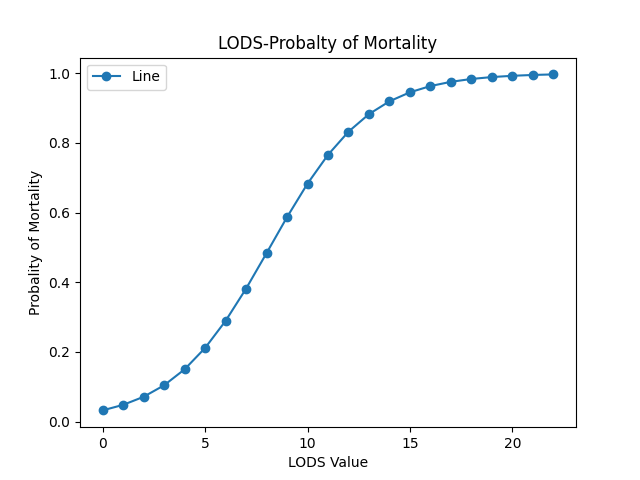
\includegraphics[width=0.8\textwidth]{thesis/img/lod_mortality_1.png}
    
  \end{center}
  \caption[LODS-Probability of Mortality]{Probability of Mortality as function of LODS value using \ref{eq:death_rate_lods}}
  \label{fig:lods_mortality}
\end{figure*}



\section{Machine Learning}
In the introduction, I introduced that machine learning imitates the way that human learns, and learns from observed data. This means that machine learning let algorithms identify patterns, relationships, and trends that humans may not be able to discern through manual analysis. Then the algorithms can apply the identified knowledge on unseen data to make predictions and decisions. 

Differ from statistics, which focuses on understanding data and inferring based on data, machine learning focuses more on model establishment and accuracy of results on prediction tasks. As a result, machine learning performs more accurate in prediction task than statistics when source dataset is large. However, machine learning models tend to be less interpretable than statistics models, because they do not impose relationships between predictors and outcomes. Machine learning has algorithms in dimensionality reduction, such as t-distributed stochastic neighbor embedding, and algorithms designed to scale efficiently with the size of the dataset. These give machine learning more capability to handle high-dimensional datasets than statistics. \parencite{Bzdok2018, Rajula2020, turin2020} In this study, I focus on the accuracy of the model and work with large dataset, so I select machine learning.

There is a branch of machine learning dealing with algorithms modeled after the structure and function of the brain's neural networks, called deep learning. It works with a set of learning techniques to model in high-level abstractions \parencite{kevin2012}. Deep learning is widely used in image recognition and natural language processing. In this study, it is used for feature extraction.

Machine Learning primarily revolves around the development of algorithms and models for decision-making. However, these decision-making processes can often be opaque or challenging to interpret, leading to the characterization of such models as "black boxes." Explainable AI (XAI) has emerged as a field aimed at enhancing the transparency and interpretability of machine learning models. It is not a distinct branch of machine learning but rather a collection of techniques and methodologies that intersect with machine learning, artificial intelligence, human-computer interaction, and ethics. \parencite{turri2022}

Given the critical importance of transparency and interpretability, explainable AI has garnered increasing attention within the machine learning in healthcare. In this study, a method from explainable AI known as SHapley Additive exPlanations (SHAP) \parencite{lundberg2017} is employed to elucidate the contribution of each feature to the model.

Here I introduce the basic concepts and methods of machine learning used in this study. 

\subsection{Supervised Training and Regression}
Machine learning is usually divided into three types, 1) \textit{supervised training}, an approach to train models that  map from inputs to outputs, 2) \textit{unsupervised training},  an approach to find "interesting pattern" in the input data, analyze and cluster unlabeled dataset 3) and \textit{reinforcement learning} which is useful in learning how to give reward and punishment. In this thesis, I focus on supervised training. \parencite{kevin2012, WANG2023}

In supervised training, the machine learning algorithm uses the labeled data to guide learning. \textit{Classification} and \textit{regression} are two most common categories of supervised training. Classification is widely used when outputs are categorical, such as Male and Female, while regression is used when labels and outputs are finitely discrete and continuous. I focus on regression in this thesis. \parencite{sagar2024}

Regression is used to predict the value of the dependent variable. It maps the relationship of the input variables, referred as \textit{features}, and the target value, referred as \textit{target}. In training process, the regression model takes the input features and give a predicted output. Then, the difference between real target value and predicted output is calculated, referred as $loss$. In most cases, the target of a model is to minimize the loss. So the model will continuously optimize the parameters of the model to reduce the loss. \parencite{sagar2024, kevin2012}

As aforementioned, the model applies relationship on unseen data. The objective of a model is performing well in the unseen data, instead of training data. Generally, to archive this target, a three-way split is performed on the dataset, training set, validation set and test set. Models are trained with training set and validated with validation set. The result of validation can be used to optimize the model hyper parameters. The test set is the unseen data to check models' performance. The goal is to maximise the performance of model in the test set. \parencite{stanford_ml}

\subsection{Underfitting and Overfitting}
According to \textcite{stanford_ml}, when models learn with training set, there are two error situations happen, $underfitting$ and $overfitting$. Under-fitting refers to that model learns too crudely between features and target. It doesn't capture the data complexities, like Figure \ref{subfig:underfitting} While overfitting refers to that model learns too complex from data, where learnt from noise and inaccurate data as well, like Figure \ref{subfig:overfitting}. Both situations will affect the model's performance on test set. Figure \ref{subfig:goodfitting} is a good fitting, that is a perfect situation in model training.
\begin{figure*}
  \begin{center}
    \subfigure[Underfitting]{
      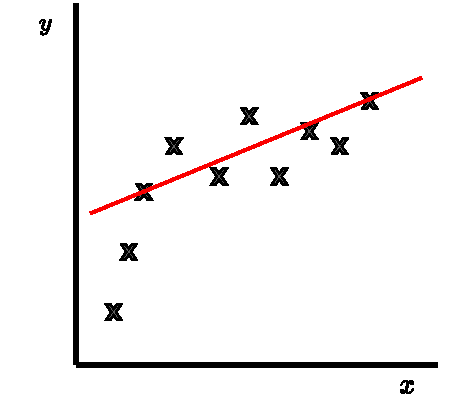
\includegraphics[width=0.45\textwidth]{thesis/img/underfitting.pdf}
      \label{subfig:underfitting}}                        
    \subfigure[Good fitting]{
      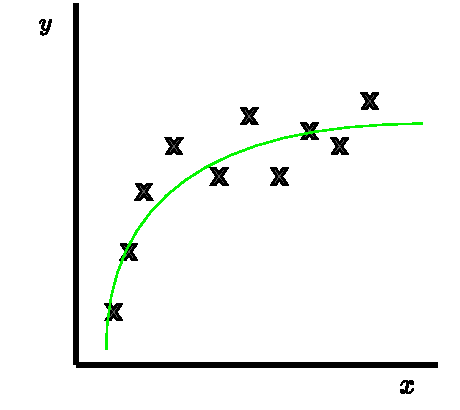
\includegraphics[width=0.45\textwidth]{thesis/img/goodfitting.pdf}
      \label{subfig:goodfitting}}                        
    \subfigure[Overfitting]{
      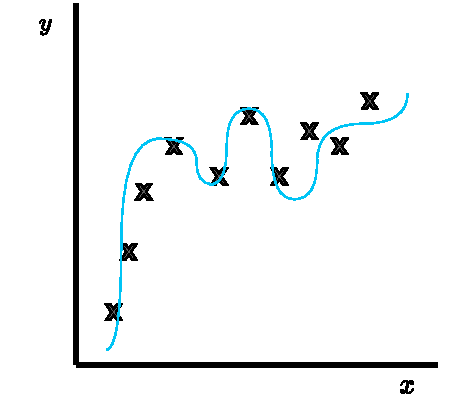
\includegraphics[width=0.45\textwidth]{thesis/img/overfitting.pdf}
      \label{subfig:overfitting}}
    \caption[Under, Good and Overfitting]{Underfitting, Goodfitting and Overfitting}
    \label{fig:different_fitting}
  \end{center}
\end{figure*}

Underfitting and overfitting can be diagnosed by comparing training error and validation error. Underfitting is associated with high error in both training and validation, while overfitting is associated with low error in training but high error in validation. Both situations will cause high error in test set, which is called generalisation error. 

The common techniques to prevent underfitting and overfitting focus on data source quality and model's hyperparameters. Regarding data source quality, increasing training data amount can improve model's ability to generalize. And increasing data complexity appropriately can improve model's ability to identify noise and details. Adjusting hyperparameters, for instance tree amount and depth in random forest, can affect model's sensitivity in noise data. 

\subsection{Machine Learning in ICU Settings}
Patients in ICU are monitored with different equipment and care workers, and some patients rely on life support machines to assist with treatment. Data produced by these equipment and machines are highly complex and large-scaled. This gives machine learning a chance to develop. In the past decades, there are many studies on applying machine learning on ICU data to support doctors' decision. According to \textcite{Kim2011}, machine learning has provided more gains than traditional statistics on outcome prediction. Some machine learning models perform real-time prediction with data from monitors \parencite{mitdavid2020, Zhale2021}. \textcite{sin2022} proposed a model in pressure ulcer prediction which could assist care workers in ICU. 

Machine learning has flexibility and scalability and is capable to analyse diverse data types in medical. But according to \textcite{ngiam2019}, it also presents unique challenges, especially in medical data preprocessing, ethical considerations, and data privacy and security. With the development of data policy in different regions, like General Data Protection Regulation (GDPR) \parencite{GDPR2016}, personal data should be highly protected in study. Due to these, some public medical database are developed for research, for example eICU Collaborative Research Database (eICU-CRD) \parencite{Pollard2018} and the Medical Information Mart for Intensive Care (MIMIC)-IV database \parencite{johnson2023}. The access to these large database gives machine learning a chance to develop in medical studies.

% Two most common categories of supervised training are classification and regression. Classification is widely used when outputs are categorical, such as Male and Female. Labels and outputs in regression are finitely discrete and continuous, respectively, such as the age a viewer of a video in YouTube. In this thesis, I focus on mapping measurements of patients’ situation to the LODS value. Typically, the measurements are referred to as features, while the LODS are referred to the target variable. Besides algorithm and model, training process also needs a notion called loss. In most cases, the machine learning tries to minimise the loss between expectation and real target in the training dataset. However, the objective of a model is not performing well in the training set, but in the unseen data. Generally, to archive this target, a three-way split is performed on the dataset, training set, validation set and test set. The goal is to maximise the performance of model in the test set. The main use of validation set is to choose the hyperparameters of the model, which are not optimized by the learning algorithm. Regularisation parameter is an important class of hyperparamenter to control under-fitting and over-fitting on training set. Under-fitting refers to that model learns too crude between predictors and targets, while overfitting refers to learning too complex. Both situation can be diagnosed by comparing training error and validation error. Underfitting is associated with high error in both training and validation, while overfitting is associated with low error in training but high error in validation. Both situation will cause high error in test set which is called generalisation error. Regularisation aims to balance the underfitting and over fitting. Bias and variance are widely checked in regression. Bias checks if the parameters entered the true parameters, and variance checks the spread level of the parameters. Both are inevitable, so the target is to balance the bias and variance to get an optimal model.
%Another way to choose hyper parameter is to perform cross validation. A common form of cross validation is K-fold validation. Instead of a single training and validation set, K folds training and validation sets are formed by partitioning the available dataset. Each set is used as validation set at a time and others are used as training set. At the end, the averaged validation error is obtained to monitor the training performance. 



\chapter{Prior Work}
\label{ch:priorwork}
Machine learning has been extensively employed in ICU severity prediction and estimation across numerous studies, each utilizing diverse prediction targets, datasets, and algorithms. In this chapter, our objective is to illuminate prior research within three pertinent categories. Firstly, I delve into existing studies concerning prediction models utilizing bedside data within ICUs, while also addressing studies akin to one experiment conducted within this thesis. Secondly, I examine research focused on the utilization of LODS and SOFA, both of which serve as organ dysfunction scores, either as targets or integral components of the model. Notably, there exists an example directly aligned with the scope of this thesis. Lastly, I delve into the utilization of Convolutional Neural Networks and XGBoost in the realm of medical-related machine learning models. 

\section{Models with bed side data in ICU}
In this section, I provide a literature survey of using bedside data in ICU related prediction models, including pediatric ICU. Electronic Health Record (EHR) data is widely used in previous efforts to predict health outcomes, which contains static or slowly evolving information, medical notes, laboratory test information, etc. However, few studies focused on bedside data, which comes from monitors. Instead of an extensive review of the studies, I focus on data process, feature extraction and results.

\textcite{mitdavid2020} conducted a study focusing on predicting the likelihood of long-time stay following intubation, leveraging continuous vital sign information alongside static clinical data. Vital signs were sourced from the Medical-Surgical ICU at Boston Children's Hospital, captured by routine bedside monitors (Philips IntelliVue MP90, Philips, Andover, Massachusetts), and recorded at a 5-second frequency using the T3 system (Etiometry, Allston, Massachusetts). The vital signs included heart rate, breathing frequency, pulse, and SPO2, supplemented by static clinical data. To address missing data gaps of $\leq$ 20 minutes in vital signs, Gaussian processes were employed for imputation, as they calculate imputed data systematically without imposing structural assumptions. Subsequently, the raw time series data from monitors were transformed into vectors of statistical features using feature-based methods. Finally, an unsupervised learning approach based on clustering strategies was applied to select features. 

Three classification studies were devised: 1) utilizing solely vital sign information for classification, 2) relying solely on static clinical data for classification, and 3) integrating both time series vital signs and static clinical data for classification. Following comparison, the third scenario demonstrated the most promising performance, achieving an area under the curve (AUC) of 0.9 with a 95\% confidence interval [0.80-0.96]. This outperformed other models designed for similar tasks, wherein the model using static clinical data alone attained an AUC of 0.73, and the model utilizing vital sign information alone achieved an AUC of 0.83. 

In \textcite{horton2022}, William and colleagues present a predictive model for impending ICU hypoglycemia. This study utilized patient data from ICU admissions at the University of Virginia Medical Center spanning from October 2013 to August 2017. The study included patients aged 18 years and older who received insulin therapy. The primary outcome considered by William and colleagues was hypoglycemia, defined as any episode of blood glucose falling below 70 mg/dL and requiring administration of 50\% dextrose injection within 1 hour.A comprehensive set of 61 vital signs, laboratory values, demographics, and continuous cardiorespiratory monitoring variables were initially selected for univariable analysis. This included measurements such as respiratory rate measured by pulse oximetry and chest impedance, as well as systolic blood pressure obtained via cuff measurement. Subsequently, 41 measurements were retained for multivariable modeling after removing the most predictable features that exhibited correlations exceeding an \textit{R}2  value of 0.9 with other features. Missing data were imputed using median values. A logistic regression model was constructed following feature selection and imputation. To assess the model's performance, a 10-fold cross-validation technique was employed.

The cross-validated AUROC of the model yielded an impressive score of 0.83, surpassing models utilizing laboratory values only (excluding glucose), vital signs only, and continuous monitoring variables only. Furthermore, an external validation was conducted using the Medical Information Mart for Intensive Care (MIMIC-III) Waveform Database Matched Subset. This subset comprises 22,317 waveform records and 22,247 numeric records for 10,282 distinct ICU patients at the Beth Israel Deaconess Medical Center. The external validation demonstrated robust performance, with an AUROC of 0.79. 

\textcite{yijing2022} proposed a real-time and interpretable model utilizing bedside vital signs monitoring to predict cardiac arrest in critically ill patients. This model was trained using data from the Medical Information Mart for Intensive Care (MIMIC-III) database. Four vital signs were collected with multi-parameter waveform data, including electrocardiogram (ECG), SpO2, invasive blood pressure (IBP), and respiratory (RESP) waveform data. Outliers were identified using the interquartile range method, considering values outside of the first and third quartiles as outliers. Missing measurements were imputed using carry-forward imputation. The preprocessed vital signs, encompassing heart rate (HR), systolic blood pressure (SBP), diastolic blood pressure (DBP), mean blood pressure (MAP), SpO2, and respiratory rate (RR), were utilized as raw features of the model, resulting in a total of 43 features. The XGBoost algorithm was employed for model training, in conjunction with three-fold cross-validation. Additionally, the authors leveraged Shapley Additive exPlanations (SHAP) values to quantify the impact of each feature. 

The model demonstrated promising results, successfully identifying 95\% of cardiac arrest patients, with 80\% of cardiac arrest cases detected 25 minutes prior to the event. However, it exhibited a 37\% error rate in non-cardiac arrest patients, resulting in an overall accuracy of 66\%. 

\textcite{gultepe2013} utilized three vital signs (temperature, respiration rate, mean arterial pressure) along with white blood count (WBC) to propose models for lactate level prediction in individuals with sepsis. Data from 741 patients, comprising 590 non-sepsis controls and 151 with sepsis, were extracted from the Electronic Health Records (EHR) of the University of California Davis Health System. The input variables consisted of vital signs and WBC, while lactate level served as the target variable. A lactate level cutoff point of 4 mmol/L was established, distinguishing high lactate levels (\textgreater4 mmol/L) from low levels.

The prediction task was executed using classification algorithms, namely Naive Bayes (NB), clustering via Gaussian Mixture Model (GMM), and Hidden Markov Model (HMM). Notably, the models demonstrated optimal performance during the second 24-hour time frame. The GMM classifier exhibited the highest mean Area Under the Curve (AUC) (µGMM=0.794, µHMM=0.709, µNB=0.664; all comparisons p\textless0.05), as indicated by the Tukey post hoc test.

Furthermore, the study explored predicting mortality risk for sepsis patients, showcasing the applicability of Support Vector Machines (SVM) classification with feature selection. Specifically, three variables—median lactate levels, median mean arterial pressure, and mean absolute deviation of respiration rate—were utilized. The resulting accuracy of 0.73 was comparable to that of other models incorporating more complex variables, underscoring the efficacy of this simplified approach.

 

\section{Organ dysfunction score related research}
This section will show literature review of studies that involved organ dysfunction scores. As this study focuses on machine learning, I only select studies that cover machine learning, ICU for adults, and organ dysfunction scores. In the first two reviews, I focus on how the organ dysfunction scores are involved. In the last, I review the whole study as it also has similar machine learning model training as this thesis.

In \textcite{zeng2021}, a blended machine learning model was developed for predicting mortality in ICU patients with sepsis. The model underwent training utilizing the eICU Collaborative Research Database and was subsequently tested on the Medical Information Mart for Intensive Care III (MIMIC-III). The organ dysfunction scores employed in this study included the Sequential Organ Function Assessment (SOFA) and the Simplified Acute Physiology Score (SAPS II), both widely recognized ICU scoring systems. During data collection, SOFA was utilized to identify consequent organ dysfunction, characterized by an acute change in SOFA scores of $\leq$ 2 points within the first 24 hours of ICU admission. Notably, SOFA was chosen for identifying organ dysfunction instead of the Systemic Inflammatory Response Syndrome (SIRS) score, aligning with recommendations from the Third International Consensus Definition for Sepsis (Sepsis-3).

The study encompassed training four distinct models, each employing different feature selection methodologies. These included a model utilizing a total of 65 variables extracted from both databases, another incorporating features selected via stepwise logistic regression with both forward selection and backward elimination, and two additional models respectively utilizing variables inherent to the SAPS II and SOFA scores.

In this study, SAPS II and SOFA were employed as benchmarks for model validation. While SAPS II has a predefined formula for calculating the probability of death, SOFA cannot be directly utilized for this purpose. Therefore, the authors devised a SOFA score-based logistic regression model, termed a refitted SOFA score, wherein the SOFA score was mapped to the predicted probability of death in the training dataset. The results indicated that the model utilizing all 65 variables and the model featuring selected variables from the same set both exhibited superior discrimination, as evidenced by their AUROCs (0.815; 95\% CI, 0.808 to 0.822 vs. 0.817; 95\% CI, 0.810 to 0.823, \textit{P} = 0.251). These performances surpassed those of the SAPS II and refitted SOFA score models.

In a study from \textcite{hatem2018} on consecutive events within patients' Electronic Health Records (EHR) data aimed at predicting deterioration in the ICU, the focus was on multiple organ failure, particularly cardiovascular and pulmonary issues. Predictions were made for events occurring three hours into the future. During model training, the worst Laboratory-based Organ Dysfunction Score (LODS), calculated as the maximum between cardiac LODS and pulmonary LODS, was utilized as the target variable.

Hatem classified the maximum LODS into two classes: Class 0 representing LODS values of 0 or 1, and Class 1 corresponding to LODS values of 3 or 5. Three models were trained for the classification task: Logistic Regression, Random Forest Classifier, and Convolutional Neural Network (CNN). The CNN model exhibited the best performance, achieving a sensitivity of 77.9\% and a specificity of 51.02\%. 

\textcite{asuroglu2021} proposed a deep learning approach was proposed to monitor sepsis onset by predicting Sequential Organ Function Assessment (SOFA) scores using seven vital signs measured over a 12-hour window in the Intensive Care Unit (ICU). These vital signs include heart rate, systolic and diastolic blood pressure, respiratory rate, oxygen saturation, Glasgow Coma Scale eye opening (GCS), and temperature. The experiments were conducted using a subset of the Medical Information Mart in Intensive Care (MIMIC) III dataset, comprising 53,423 ICU records of patients aged over 15 from 2001 to 2012 at Beth Israel Deaconess Medical Center (BIDMC) in Boston, Massachusetts. Asuroglu's experiments utilized 5,154 samples that met three additional inclusion criteria: (1) predictability of sepsis onset time, (2) availability of at least one measurement for each vital sign within 12 hours prior to predicting onset time, and (3) determination of an artificial onset time, including patients without sepsis. These samples were used to train a model to predict SOFA scores, which are used for sepsis evaluation. Probabilistic Principal Component Analysis (PPCA) was employed to impute missing values in the dataset, utilizing a combination of Principal Component Analysis (PCA) with a probabilistic approach and Expectation-Minimization method.

To achieve the goal, Asuroglu combined Convolutional Neural Networks (CNN) features with the Random Forest (RF) algorithm. CNN served as a feature extraction tool, while Random Forest made the final decision. Prediction performance was assessed using Correlation Coefficient (CC), Mean Absolute Error (MAE), and Root Mean Square Error (RMSE). The model demonstrated superior performance compared to other models such as Bi-LSTM and Linear Regression, achieving an RMSE of 1.23, MAE of 0.659, and CC of 0.863.

\section{Decision Tree based algorithm applied on medical data}
This section will show a short literature survey of algorithms used in ICU-related machine learning. The main algorithms used in this thesis are Convolutional Neural Network (CNN) and XGBoost. However, CNN is widely used in medical image classification and object detection due to its powerful visual imagery analyzing ability. There is a research, from \textcite{asuroglu2021}, that used CNN for feature extraction, covered in the previous section. So this section will focus on using a decision tree based model in ICU-related machine learning study, mainly on how the model was trained with medical data.

In the study conducted by \textcite{rahman2021}, early prediction of hemodynamic interventions one hour into the future in the ICU was investigated. Rahman and colleagues developed a model utilizing the eICU Research Institute (eRI) database, employing an ensemble of decision trees to derive a real-time risk score. The dataset comprised 33 variables, including vital signs, laboratory measurements, blood gas measurements, and ventilation settings, which were fed into an Abstain-Boost model. This model integrates boosting principles with the capability to abstain from making predictions on difficult or uncertain instances.

The trained model consists of 33 univariable classifiers, each corresponding to a variable, with each classifier comprising decision trees of depth one and outputting a real value. The learning rate of the model was set to 0.1, and training was conducted over 200 rounds of boosting. The variable-wise risks were aggregated and transformed using sigmoid to obtain the final result. Additionally, Platt scaling was applied to calibrate the predicted probabilities.

During model training, efforts were made to mitigate bias by merging invasive and noninvasive blood pressure measurements, imputing missing values with the mean value, and adding missing variable indicators to the model. However, the latter action was later discarded to enable the model to learn purely from physiological data, rather than incorporating patterns of clinical practice. Consequently, the model exhibited an area under the curve (AUC) of 0.82, successfully predicting 52\% of hemodynamic interventions with a lead time of one hour.


In the study conducted by \textcite{liu2022}, the focus was on predicting mortality in the ICU based on a time-incorporated Sequential Organ Function Assessment (SOFA) score. Four machine learning algorithms were employed: eXtreme Gradient Boosting (XGBoost), Support Vector Machines, Random Forest, and Logistic Regression. Among these, XGBoost demonstrated the best performance.

The study utilized the Medical Information Mart for Intensive Care (MIMIC-III) version 1.4 and the eICU-Collaborative Research Database (eICU-CRD) version 2.0 as the training set, while a mixed dataset comprising MIMIC-IV version 1.0 and a local dataset from Nanjing Jinling Hospital Surgery ICU (SICU-JL) database served as the test set.

The model collected patients' demographic information and clinical data related to the SOFA score as input features, with patient outcome serving as the output. Training the model occurred in three steps. Initially, only the total SOFA score and sub-scores at each time point were included, resulting in the T-SOFA M1 model. Subsequently, the authors incorporated time dimensions to train the T-SOFA M2 model. Finally, age was added as an additional feature for training.

The final result of the XGBoost model yielded an area under the curve (AUC) of 0.8, outperforming the other machine learning algorithms utilized in the study.

 


\begin{comment}
Mathematics and machine learning have been brought to ICU severity prediction and estimation in many research, however, most of them focus on combine laboratory and vital sign measurements together to predict mortality. There are some studies that use bedside data to estimate or predict patients' situation.
 
\textcite{johnson2013} used 10 bedside variables to propose a score system called Oxford Acute Severity of Illness Score (OASIS) to estimate patients' situation in the first day of ICU stay, include pre-ICU length of stay, age, Glasgow Coma Scale (GCS), heart rate, mean arterial pressure (MAP), respiratory rate, temperature, urine output, ventilated or not and elective surgery or not. It uses the worst value of the variables in the first 24 hours in ICU stay, which conduct a scale from 0 to 73. OASIS also includes an equation to convert score to mortality. The objective of the study was to use a machine learning technique which is called particle swarm optimization to reduce the number of parameters collected in Acute Physiology, Age, and Chronic Health Evaluation (APACHE) IV system with no predictive accuracy lost. The data of this study, 81,807 admissions, was a subset of data obtained from 86 ICUs at 49 hospitals that had installed an APACHE IV system from January 1, 2007 to September 15, 2011. Patients with burn, stay in ICU less than 4 hours and younger than 16 are excluded from the dataset. Posttransplant patients, other than hepatic or renal transplantation, are excluded from the research. there are 8613 admissions were removed because of the missing variables, resulting in a final cohort of 72,474 admissions, which was divided into development dataset (39,070 admissions), internal validation dataset (9,786 admissions) and external validation dataset (23,618 admissions). Genetic Algorithm (GA) was used to select variables, and particle swarm optimization was used to determine the weight assigned to each variable. A research in China validated that OASIS have better accuracy than Sequential Organ Function Assessment (SOFA) and Logistic Organ Dysfunction Score (LODS) in mortality prediction of patients with sepsis in ICU \parencite{hu2020}. \textcite{el-manzalawy2021} used 10 variables of OASIS and machine learning model to propose a new OASIS+ score system.

\end{comment}

\section{Discussion of Prior Work}

Previous research has shown that relying solely on bedside data does not achieve performance levels comparable to using a combination of bedside and EHR data. However, increasing the number of variables can lead to a more complex model that is less interpretable, affecting its usability in a clinical setting. An ideal clinical model should strike a balance between simplicity and high accuracy. 

Organ dysfunction scores are primarily used as a baseline for evaluating models, but their longstanding use in clinical practice gives them an important role in supporting doctors' decision-making processes. Some scores are even considered diagnostic indicators. Integrating these scores into machine learning models can provide doctors with evidence-based support for decisions and enhance the usability of machine learning models in clinical settings. This integration addresses a gap in machine learning research that focuses on organ dysfunction scores, which this study aims to fill. 

Convolutional Neural Network (CNN) is recognized as a highly effective algorithm for analyzing grid-like matrix data, capable of capturing intricate details. In medical research, CNN has been utilized for feature extraction. XGBoost is known for its strong performance in prediction tasks and has shown superiority over other algorithms like random forest. In this study, I aimed to leverage the strengths of both algorithms by using CNN for feature extraction and XGBoost for prediction, to evaluate their combined performance. 


\chapter{Methods}
\label{ch:methods}
This chapter will introduce the dataset and algorithms used in this study. Algorithms cover these used in feature reduction, missing data imputation, model training and evaluation.

\section{Dataset}
The dataset used in this study should simulate the hospital environment as completely as possible, which includes all departments instead of a set of ICUs from many hospitals. The reason is that for one hospital, all equipment of each vital sign monitor is mostly same model, so I can ignore the difference in measurements from equipment. Most patients are transferred from another department to ICU, in which situation, in the first several hours of ICU stay, there may not be measurements. So I should try to collect data from the records in the original department. Comprehensiveness and preprocessed level are two criteria when selecting a dataset. Moreover, I wanted to use data from a multiracial country so that I could reduce the bias of race in this study. I selected the Medical Information Mart for Intensive Care (MIMIC)-IV database version 2.2 \parencite{johnson2023} in this study. 

The MIMIC IV dataset is the updated version of the MIMIC III created in 2020. It comprises deidentified health-related data from patients who were admitted to the critical care units of the Beth Israel Deaconess Medical Center (BIDMC) in 2008-2019 in Boston Massachusetts. The dataset consists of 73,181 ICU stay records; vital sign and laboratory measurements of these records are all included. MIMIC IV data is de-identified, and patient identifiers have been removed according to the Health Insurance Portability and Accountability Act (HIPAA) Safe Harbor provision.A waiver of informed consent and approved the data sharing initiative by the Institutional Review Board at the Beth Israel Deaconess Medical Center, who reviewed the collection of patient information and creation of the research resource. \parencite{johnson2023}

MIMIC-IV is created in 3 steps, 1) acquisition, to acquire the data from clinic system and filter data from all tables to only rows related to patients, 2) preparation, to reorganize the data for better facilitate retrospective data analysis and process doesn't have cleaning step, to ensure the data reflects a real-world clinical dataset, 3) deidentify, to remove patient identifiers as stipulated by HIPAA and assign a \textit{stay\_id} to each single date so that a single patient has internally consistent data. MIMIC-IV has 2 modules; hosp and icu. The Hosp module contains all data from the hospital wide electric health record, covers patient and admission information, laboratory measurements, microbiology, medication administration, and billed diagnoses. This uses ICU module to finish the experiment. The ICU module provides information from the clinical information system used within the ICU, MetaVision (iMDSoft), covers intravenous administrations, ventilator settings, and other charted items. MetaVision tables were denormalized to create a star schema. the \textit{icustays} and \textit{d\_items} tables link to a set of data tables,  suffixed with "events". All event tables contain a \textit{stay\_id} column to identify the associated ICU patient in \textit{icustays}. The \textit{stay\_id} is used to search and connect all the events record in this thesis. 

\section{Feature Correlation and Reduction}
When training a machine learning model, there are commonly many features collected in dataset. However, not all of them are needed. Those exhibiting a strong correlation with the target variable are often utilized during training, while those with low correlation are typically disregarded. Correlation coefficients are employed to assess the relationship between features and the target variable. In instances where two features display high correlation, redundancy may arise, prompting the removal of one feature during model training.

The correlation coefficient is a statistical measure indicating the strength and direction of the linear relationship between two variables, illustrating whether they tend to move together at a constant rate. It ranges from -1 to 1, where a value of 0 suggests no correlation. A coefficient greater than 0 signifies a positive correlation, while a coefficient less than 0 suggests a negative correlation. The magnitude of correlation is denoted by the absolute value of the coefficient. Here, I introduce two correlation coefficients. \parencite{acuk2023, Schober2018}

\subsection{Pearson Correlation}
The Pearson correlation coefficient \parencite{acuk2023, Schober2018}, denoted by "r," serves as a measure of the relationship between two continuous variables, commonly employed to assess linear relationships. It signifies that as one variable increases, the other variable will also increase (positive correlation) or decrease (negative correlation) accordingly. The value of the Pearson correlation coefficient represents the strength of this relationship and is extensively utilized to gauge the correlation between two variables. Nonetheless, it is crucial to note that the Pearson correlation coefficient is highly sensitive to outliers, which can potentially distort the interpretation of the relationship. The formula of Pearson Correlation is
\begin{equation}
  r =
  \frac{ \sum_{i=1}^{n}(x_i-\bar{x})(y_i-\bar{y}) }{%
        \sqrt{\sum_{i=1}^{n}(x_i-\bar{x})^2}\sqrt{\sum_{i=1}^{n}(y_i-\bar{y})^2}}
\end{equation}
where $x_i$ is data points of one variable, $y_i$ is data point of another variable, $\overline{x}$ is the mean of $x$ variable, and $\overline{y}$ is the mean of $y$ variable. Besides assessing correlation, Pearson correlation is useful for evaluating the effectiveness of machine learning models by comparing values predicted by models and real values. \parencite{kirk2021} 

\subsection{Spearman Correlation}
Spearman correlation coefficient \parencite{acuk2023, Schober2018}, denoted by \(\rho\), serves as a measure of the monotonic relationship between two variables. It is particularly suitable for ordinal or non-normally distributed data. Unlike the Pearson correlation coefficient, which is based on the actual coefficient value, the Spearman correlation coefficient is derived from the ranks of the data. It evaluates whether variables change together, without requiring a constant rate of change. The formula of Spearman Correlation is
\begin{equation}
    \rho = 1- {\frac {6 \sum d_i^2}{n(n^2 - 1)}}
\end{equation}
where \textit{d} is the difference between the ranks of corresponding variables and \textit{n} is the number of data points. Spearman correlation is robust to outliers as it operates on ranks rather than actual data values. However, the precision of the Spearman correlation coefficient is influenced by the number of data points used in the calculation, meaning it tends to be less precise with smaller datasets compared to larger ones. It is commonly utilized when the relationship between variables cannot be assumed to be linear.

In this study, to get a good correlation measurement, both coefficients are used to check the relationship between variables and target, LODS value.

\section{Missing Data Imputation}
In real world, missing data is a common problem in machine learning. Most models do not work correctly when input data contains empty elements.

There are three types of missing data, classified by \textcite{rubin1976}

1. Missing Completely at Random (MCAR) refers to a scenario where the probability of data being missing is consistent across all data points and is independent of both known values and the missing values themselves. This implies that the causes of missing data are unrelated to the actual data. For example, no heart rate was measured for a patient due to the broken equipment. The probability of any patients being affected is uniform. In such cases, the missing data can be regarded as following the same distribution as the known values, thereby simplifying many complexities, aside from the obvious loss of information.

2. Missing at Random (MAR) describes a situation where the probability of data being missing is uniform only within groups defined by observed data and depends solely on the observed values rather than the values themselves. MAR encompasses a broader range than MCAR. For example, young people take less healthcare service than old people. As a result, healthcare data of young people is less likely recorded than older people. MAR is more encompassing than MCAR, leading modern missing data methods to typically begin with the MAR assumption.

3. Not Missing at Random (NMAR) refers to a scenario where the probability of data being missing is unknown and depends on the value of the variable itself. In NMAR situations, missing data likely holds valuable information. For example, Lower educational attainment, poor economic conditions, and long distances to healthcare facilities may lead to some individuals using healthcare services less frequently than usual. The causes of these cases are related to unknown characteristics. NMAR poses a more intricate challenge compared to the other two cases. Strategies for handling NMAR involve seeking additional data to understand the underlying causes or conducting what-if analyses to evaluate the sensitivity of results under various scenarios.\parencite{vanbuuren2018, Pedersen2017}

To keep the training process work smoothly, the NMAR and MAR in dataset should be imputed. In this study, I used two missing data imputation methods, linear interpolation and Probabilistic Principal Component Analysis (PPCA).

\subsection{Linear Interpolation}
Linear interpolation is an method for data interpolation. It bases on the two data points adjacent to the target point to estimate the data value in the data sequence, as Figure \ref{fig:linear_impute_fig}. With the simplest linear interpolation, the target points are joined by straight line segment. As a result, each segment is interpolated independently and segments discontinue at each point. \parencite{huang2021, paul1999}
In contrast, a smoother interpolating function is desirable. Cosine interpolation and Cubic interpolation are two simple methods \parencite{paul1999}.

\begin{figure*}
  \begin{center}
    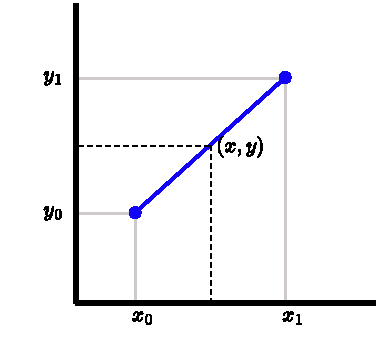
\includegraphics[width=0.7\textwidth]{thesis/img/linear_impute.pdf}
  \end{center}
  \caption[Linear Interpolation]{Linear Interpolation to calculate missing data between two known data points of one-dimension}
  \label{fig:linear_impute_fig}
\end{figure*}

\subsection{Probabilistic Principal Component Analysis}
Probabilistic Principal Component Analysis (PPCA) is a probabilistic extension of Principal Component Analysis (PCA). Here is an instruction of PCA and PPCA, comes from \textcite{lindsay2002} and \textcite{tipping2002}.
Principal Component Analysis, developed by Karl Pearson in 1901, is a powerful dimensionality reduction technique that aims to transform high-dimensional data to low-dimensional space without losing most of the variance in the data \parencite{mackiewicz1993}. The variables in low-dimensional space are called principal components, which are linear combinations of original variables. This is achieved by finding the directions along which the variance of the data is maximized. It is used for data compression, dimensionality reduction and data visualization. 

Standardization ensures that all variables are on same scale (normally 0 - 1) and prevents variables with large magnitudes from dominating the analysis, by subtracting the mean and dividing by the standard deviation of each variables. For each feature $X_i$ in the dataset, standardized value $Z_i$ should be calculated with: %\ref{eq:ppca_standardized_value}
\begin{equation}
    \label{eq:ppca_standardized_value}
    {Z_i} = {\frac {{X_i}-{\mu_i}}{\sigma_i}}
\end{equation}
where $\mu_i$ is the mean of feature $X_i$ and $\sigma_i$ is the standard deviation.

Covariance Matrix provides relationship info between each pair of variables. It indicates how much two variables vary together, and a positive covariance means two variables tend to increase or decrease together, while a negative indicates an inverse relationship. Covariance Matrix is calculated on the standardized dataset by 
\begin{equation}
    C = \frac{1}{n}\sum\limits_{k=1}^n (x_k -  m)\;( x_k -  m)^T
\end{equation}
where $n$ is the number of observations and $m$ is the mean vector of the standardized data.

Eigenvalue Decomposition involves decomposing the covariance matrix into eigenvectors, which represent the directions of maximum variance in the data, and eigenvalues, which indicate the magnitude of variance along these directions. Each eigenvector corresponds to a principal component, and the associated eigenvalue represents the amount of variance explained by that component.

The Selection of Principal Components in PCA involves sorting the eigenvalues in descending order and selecting the top k eigenvectors (considered as principal components) corresponding to the largest eigenvalues. These principal components capture most of the variability.

Projection in PCA involves projecting the original data onto a new orthogonal basis formed by the selected principal components. This transformation creates a new dataset where each observation is represented by a linear combination of the principal components.

In Probabilistic Principal Component Analysis (PPCA), the principal components are treated as random variables. The observed data are generated by a linear transformation of a lower-dimensional latent space plus Gaussian noise. The latent space is of lower dimensionality than the original data space and captures the essential features of the data. Maximum likelihood estimation or Bayesian inference is used to estimate the parameters of the model, including the latent variance space and the noise variance. With the estimated parameters, the latent space can be utilized for dimensionality reduction.

With a data set $X$ consisting of $N$ data points, each of dimension $D$. And the target lower-dimensional latent space $Z$ of dimension $M$ ($M$ < $D$). So, each data point $x_n$ is generated from $z_n$ through a linear transformation plus Gaussian noise:
\begin{equation}
    {x_n} = {W}{z_n}+{\mu}+{\epsilon _n}
\end{equation}
where $W$ is a $D$ $\times$ $M$ matrix of the loading vectors, representing the linear transformation from the latent space to the observed data space, $z_n$ is a $M$ -dimensional latent variable associated with n-th data point, $\mu$ is the mean of the data, and $\epsilon _n$ is Gaussian noise with mean zero and covariance matrix.
In PPCA, the latent variables $z_n$ are assumed to follow a Gaussian distribution:
\begin{equation}
    {z_n} \sim {\mathcal{N}}(0, {I})
\end{equation}
where $I$ represents the identity matrix, which is a square matrix with ones on the diagonal and zeros elsewhere. Once the $W$, $\mu$, and $\sigma ^2$ are estimated by maximizing the log-likelihood function, the latent space $Z$ (a $M$$\times$ $N$ matrix containing the latent variables for all data points) can be obtained by:
\begin{equation}
    {Z} = {W^T}{({W}{W^T}+{\sigma ^2}{I})^{-1}}({X}-{\mu}{1^T})
\end{equation}
where 1 is a column vector of ones.

To impute the missing data $x_{ij}$ in the observed data matrix $X$, the first step is to estimate the corresponding latent variable $z_{ij}$ with the estimated loading matrix $W$ and the latent space $Z$. Then reconstructing the missing entry  $x_{ij}$ can be done by
\begin{equation}
    {x_{ij}} = {W_j}{z_{ij}}+{\mu _j}
\end{equation}
where $W_j$ is the $j$ -th column of $W$ and $\mu_j$ is the $j$-th element of the mean vector $\mu$.


\section{Models}
In this section, I introduce two primary algorithms utilized in this study: Extreme Gradient Boosting (XGBoost) and Convolutional Neural Network (CNN). XGBoost is employed for prediction due to its predictive capabilities. CNN is employed for feature extraction, leveraging its capacity to analyze grid-like matrices effectively.

\subsection{Extreme Gradient Boosting}
Decision trees are powerful non-parametric methods for classification and regression tasks which produce a recursive binary partitioning of the feature space. They build a flowchart-like tree structure where nodes represents features, branches represents decisions and leaf node represents the outcomes. When classifying new instances, a decision tree locates the area where the instance lies and take a majority vote inside the area to determine the result, based on the training set, which results it low bias and high variance. Extreme Gradient Boosting (XGBoost) is an ensemble of decision trees using gradient boosting. In the following, I examine how XGBoost actually works, according to \textcite{song2015, chen2016, mitchell2017, hastie2009, stanford_ml, geek_xgboost}

Start with decision trees. Each tree is constructed by splitting the training data into subsets recursively based on attribute selection measures until the tree met a stopping criteria, such as the depth of a tree. Attribute selection measure (ASM) is used to evaluate the usefulness of different attributes for splitting a dataset, the goal of which is to determine the best attribute that will create the most homogeneous subset of data after splitting, thereby maximizing the information gain. This process is repeated in a recursive manner, called recursive partitioning, on each derived subset. When the subset at a node all has the same target value or when splitting does not add value, the recursion is completed. There are several commonly used attribute selection measures:

Entropy, is the measure of the uncertainty or randomness in a set of elements, based on the distribution of class labels in the dataset. Entropy of each classified subset ${D}$ is calculated as
\begin{equation}
    Entropy(D)=-\sum_{i = 1}^C {p_i} \log _2 {p_i}
\end{equation}
where ${p_i}$ is the proportion of the data points that belong to class ${i}$ in subset ${D}$ , and ${C}$ is the number of classes. ${p_i}$ is calculated with
\begin{equation}
    p_i = \frac{1}{n} \sum I(y=i)
\end{equation}
where ${n}$ is the amount of data points in subset.
A high entropy indicates a high maximum uncertainty. Therefore, the even distribution of class labels has the highest entropy. In contrast, low entropy indicates low randomness of the dataset. So, a completely homogeneous dataset has entropy value 0. Entropy is used to evaluate the the quality of a split, whose goal is to select attribute that minimizes the entropy of the resulting subset.

Gini Impurity quantifies the likelihood of incorrectly classifying a randomly chosen element if it was randomly labeled based to the distribution of class labels. It is calculated as 
\begin{equation}
    Gini(D) = 1-\sum_{i=1}^C {p_i}^2
\end{equation}
where ${p_i}$ is the proportion of the data points classified as ${i}$ in subset ${D}$, and ${C}$ is the number of classes. A lower Gini Impurity indicates more homogeneous, that a subset is predominately composed of data points belonging to same class, than a higher one. Moreover, information gain is also a commonly used measurement in decision tree algorithm of the reduction in entropy results from a split.

Decision tree analyses the data set to predict its classification. It commences from the root node, the topmost node and starting point in a tree, where the algorithm compares the value of the root attribute and the attribute of the record in the actual data set. Then the algorithm proceeds to follow the branch and move to the next node. It repeats this action on each subsequent node until the leaf nodes of the tree. In each node, the algorithm finds the best attribute in the dataset with attribute selection measure. The total time of training a decision tree, include training and test is ${O_{(ndf)}}$, where ${n}$ is the amount of examples, ${f}$ is the feature amount and ${d}$ is the depth of the tree. 
Decision trees are simple to understand as it follows the same process as a human makes decisions in real-life. Figure \ref{fig:decision_tree} shows an example of decision tree structure. Also, no domain knowledge or parameter setting is required to construct a decision tree, therefore it is appropriate for exploratory knowledge discovery. In those cases where domain knowledge is already known, decision trees can also be constructed by conducting interviews with experts and manually creating them. As its calculation focuses on the outcome of each split instead of the inputted features and it commonly process one attribute in each node, it can handle high-dimensional data. But a decision tree may have over-fitting issue due to its inherent nature of complex and highly branching structure to fit training data closely, especially with limited data and deep trees without depth limit, which memorize noise and outliers in the training data and grow until it perfectly fits the training data. Moreover, decision trees are sensitive to small variations in the training data, which causes decision trees to be prone to high variance.

\begin{figure*}
  \begin{center}
    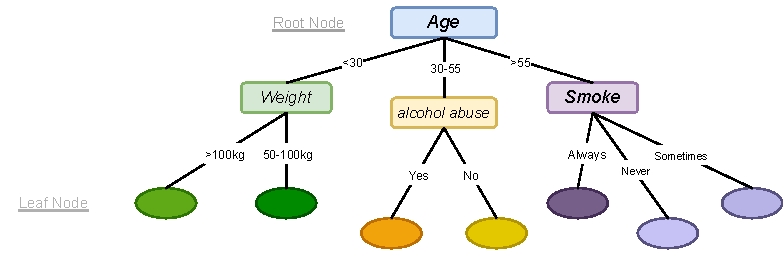
\includegraphics[width=1\textwidth]{thesis/img/decision_tree.pdf}
  \end{center}
  \caption[Decision Tree]{An example of Decision Tree Structure}
  \label{fig:decision_tree}
\end{figure*}

To address some limitations of individual decision trees and improve the overall performance of a model, ensemble decision trees are created. Bagging and boosting are two common ensemble methods. Bagging ensembles decision trees that are trained in parallel on random subsets of the original dataset and then aggregates their individual results, by voting for classification tasks or averaging for regression tasks, to form a final result. This means that some instances may be repeatedly selected, however, some may be not selected at all, which introduces further randomness and decorrelation between trees. Also with the random selection of instances, the probability of overfitting is minimized and the stability is increased as the impact of outliers and noise are reduced. Random forest is a common used powerful tool based on bagging.

Boosting is an iterative ensemble learning technique where decision trees are sequentially trained to correct the errors from previous trees. In each iteration, the new tree focuses on the instances that are misclassified or have high residuals by the previous trees and assigns those instances higher weights to emphasize their importance, while the correctly classified instances receive lower weights. This adaptive weighting scheme lets boosting to focus on the most challenging instances, gradually improving the overall performance of the ensemble. When combining predictions, boosting commonly uses weighted averaging, where the predictions of each decision tree are weighted by its performance during training, in regression task. Alternatively, in classification tasks, boosting uses a weighted majority vote where the weight of each tree depends on its accuracy in training. And it also has the advantages, as bagging, that minimizing the probability of overfitting and increasing the stability. Gradient boosting, derived from boosting, builds the ensemble sequentially by training each decision tree with the residuals of the previous tree's predictions. It optimizes a loss function by minimizing the errors of the ensemble on the training data. Regularization is also applied in boosting algorithm to prevent overfitting. XGBoost is based on gradient boosting, which ensembles regression trees, a type of decision tree used for regression tasks.

Here I explain mathematics theory of XGBoost. For a given data set with $m$ features and $n$ examples $D = \{(x_i, y_i)\}(|D|=n, x_i \in \mathbb{R}^m, y_i \in \mathbb{R})$ , the prediction is sum of each tree, in the form
\begin{equation}
    \hat{y}_i=\phi\left(\mathbf{x}_i\right)=\sum_{k=1}^K f_k\left(\mathbf{x}_i\right), \quad f_k \in \mathcal{F}
\end{equation}
where $K$ is the amount of trees, and $\mathcal{F}=\left\{f(\mathbf{x})=w_{q(\mathbf{x})}\right\}\left(q: \mathbb{R}^m \rightarrow T, w \in \mathbb{R}^T\right)$ is the space of regression trees. Here, $T$ is the number of leaves in a tree and $q$ represents the structure of the tree. $f_k$ represents each independent tree structure $q$ and leaf weights $w$, then the weight of $i$-th leaf is represented with $w_i$. The objective is to minimized the following
\begin{equation}
    \begin{gathered}
\mathcal{L}(\phi)=\sum_i l\left(\hat{y}_i, y_i\right)+\sum_k \Omega\left(f_k\right) \\
\text { where } \Omega(f)=\gamma T+\frac{1}{2} \lambda\|w\|^2
\end{gathered}
\end{equation}
where $l$ is the loss function that measures the difference between the target $y_i$ and the prediction $\hat{y_i}$. The second part $\Omega$ is the regularization parameter, that is used to smooth the final learnt weights, to avoid over-fitting. Instead of learning all trees at once, the additive strategy is applied here to minimize the loss, summarised as below:
\begin{equation}
    \begin{aligned}
& \hat{y}_i^{(0)}=0 \\
& \hat{y}_i^{(1)}=f_1\left(x_i\right)=\hat{y}_i^{(0)}+f_1\left(\mathbf{x}_i\right) \\
& \hat{y}_i^{(2)}=f_1\left(\mathbf{x}_i\right)+f_2\left(\mathbf{x}_i\right)=\hat{y}_i^{(1)}+f_2\left(\mathbf{x}_i\right) \\
& \cdots \\
& \hat{y}_i^{(i)}=\sum_{k=1}^i f_k\left(\mathbf{x}_i\right)=\hat{y}_i^{(t-1)}+f_i\left(\mathbf{x}_i\right)
\end{aligned}
\end{equation}
Then, combine this to the objective function and apply taylor series expansion, the objective function will be:
\begin{equation}
    \mathcal{L}(\phi)=\sum_{i=1}^n\left[l\left(y_i, \hat{y}_i^{(t-1)}\right)+q_i f_i\left(x_i\right)+\frac{1}{2} h_i f_i^2\left(x_i\right)\right]+\Omega\left(f_i\right)
\end{equation}

where $g_i=\partial_{\hat{y}^{(t-1)}} l\left(y_i, \hat{y}^{(t-1)}\right)$ and $h_i=\partial_{\hat{y}^{(t-1)}}^2 l\left(y_i, \hat{y}^{(t-1)}\right)$. Then apply the regularization term which is defined earlier, the objective function becomes:
\begin{equation}
    \begin{aligned}
& \mathcal{L}(\phi) \approx \sum_{i=1}^n\left[g_i w_{q\left\{w_j\right)}+\frac{1}{2} h_i w_{q\left(i_i\right)}^2\right]+\gamma T+\frac{1}{2} \lambda \sum_{j=1}^T w_{i j}^2 \\
= & \sum_{j=1}^T\left[\left(\sum_{i \in I_j} g_i\right) w_j+\frac{1}{2}\left(\sum_{i \in I_j} h_i+\lambda\right) w_j^2\right]+\gamma T \\
= & \sum_{j=1}^T\left[G_j w_j+\frac{1}{2}\left(H_j+\lambda\right) w_j^2\right]+\gamma T
\end{aligned}
\end{equation}
where $G_j=\sum_{i \in I_j} g_i $ and $H_j=\sum_{i \in I_j} h_i$. The $w_j$ are independent of each other, the optimal weight $w_j^*$ of a fixed tree is
\begin{equation}
w_j^*=-\frac{G_j}{H_j+\lambda}
\end{equation}
and the corresponding optimal value is calculated by
\begin{equation}
\mathcal{L}(\phi)=-\frac{1}{2} \sum_{j=1}^T \frac{G_j^2}{H_j+\lambda}+\gamma T
\end{equation}


\subsection{Convolutional Neural Networks}
All the aforementioned models have a simple two-layer architecture of the form input directly to output. However, there is a subset of machine learning, called deep learning, that uses multi-layer neural networks to mimic the complex decision-making process of human brain. Neural networks make up the backbone of deep learning. Here I start from neural network, according to \textcite{stanford_ml, stanford_cnn, xinyu2019, yamashita2018, veena2024}. 

\begin{figure*}
  \begin{center}
    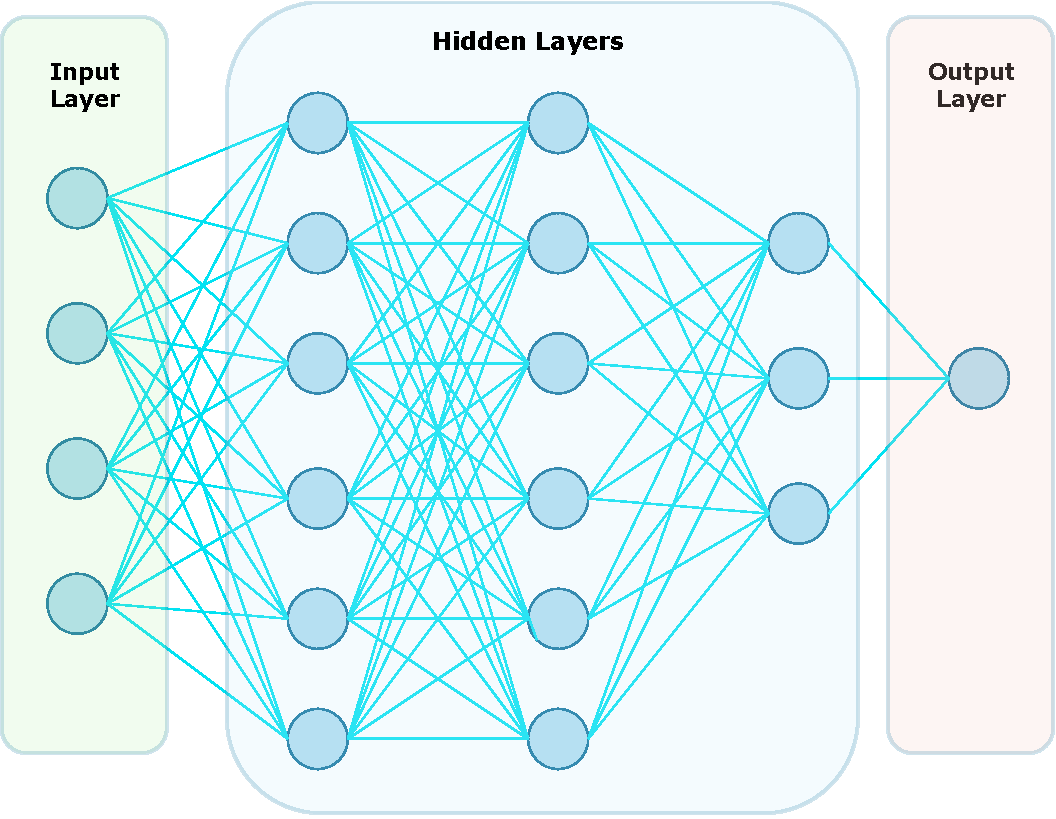
\includegraphics[width=1\textwidth]{thesis/img/neural_network.pdf}
  \end{center}
  \caption[Neural Network]{Neural Network Structure}
  \label{fig:neural_network}
\end{figure*}

Inspired by the structure and function of the brain, a neural network is a computational model that consists of  interconnected nodes or neurons, which are mathematical functions that perform a computation based on inputs and produce an output, in a layered structure. The layers between input and output layers are referred as hidden layers. Neurons inside each layer are not connected, but connected with neurons in subsequent layer through weighted connections. Each connection has an associated weight that determines the strength of the connection, as Figure \ref{fig:neural_network}. The first step to start a basic feedforward neural network is initialization, where the weights $W$ are initialized randomly and bias $b$ are initialized to zeros. The second step is forward propagation, which passes the input data through each layer of the network, performs computations and produce an output. After data is inputted, the weighted sum of inputs for each neuron is computed in the hidden layers and output layer with
\begin{equation}
    z^{(l)}=W^{(l)} \cdot a^{(l-1)}+b^{(l)}
\end{equation}
where $z^{(l)}$ is the weighted sum of inputs for layer $l$, $W^{(l)}$ is the weight matrix for layer $l$, $a^{(l-1)}$ is the output of the previous layer and $b^{(l)}$ is the bias vector for layer $l$. An activation function applies to the weighted sum $z^{(l)}$ to get an output of each neuron:
\begin{equation}
    a^{(l)}=\sigma\left(z^{(l)}\right)
\end{equation}
The most common activation functions are reLU, tanh, softmax and sigmoid. They are used depending on the type of layer and task. In this study, I used reLU. Applying an activation function will introduce non-linearity into the network, which can capture complex patterns as the real-world datasets exhibit complex relationships that can not be modeled only by linear functions, and break symmetry in the network to prevent all neurons from learning the same representation. This process will be applied on each neuron of each hidden layer and output layer, and produce a predicted result $\hat{y}$ to compute loss between it and the actual $y$ with loss function $L(\hat{y}, y)$, which is the third step. One commonly used loss function is Mean Squared Error:
\begin{equation}
\label{eq:mse}
    M S E=\frac{1}{n} \sum_{i=1}^n\left(y_i-\hat{y}_i\right)^2
\end{equation}
where $n$ is the amount of examples. The objective is to minimize the loss. To archive this, backpropagation is applied by adjusting the weights and biases, typically with gradient descent. It starts from the output layer to compute the gradient of the loss:
\begin{equation}
    \delta^{(L)}=\frac{\partial L}{\partial a^{(L)}} \cdot \sigma^{\prime}\left(z^{(L)}\right)
\end{equation}
where $\frac{\partial L}{\partial a^{(L)}}$ is the gradient of loss function with respect to the activations, $\sigma^{\prime}$ is the derivative of the activation function, and $z^{(L)}$ is the weighted sum of inputs to the output layer. The same process is propagated through each layer to compute the gradient of the loss function with respect to the activations of the previous layer and the parameters of the current layer:
\begin{equation}
    \begin{aligned}
& \delta^{(l)}=\left(\left(W^{(l+1)}\right)^T \cdot \delta^{(l+1)}\right) \cdot \sigma^{\prime}\left(z^{(l)}\right) \\
& \frac{\partial L}{\partial W^{(l)}}=\delta^{(l)} \cdot\left(a^{(l-1)}\right)^T \\
& \frac{\partial L}{\partial b^{(l)}}=\delta^{(l)}
\end{aligned}
\end{equation}
where $\delta^{(l)}$ is the loss gradient at layer $l$. Then gradient descent is used to update parameters:
\begin{equation}
    \begin{aligned}
& W^{(l)}=W^{(l)}-\alpha \frac{\partial L}{\partial W^{(l)}} \\
& b^{(l)}=b^{(l)}-\alpha \frac{\partial L}{\partial b^{(l)}}
\end{aligned}
\end{equation}
where $\alpha$ is the learning rate. The whole process, include forward propagation, backpropagation, and parameter update, is iterated to decide final parameters which produce the minimum loss and output.

Convolutional Neural Network (CNN) is the extended version of feed forward neural network primarily used for analyzing visual imagery, and predominantly used to extract the feature from the grid-like matrix dataset, such as time-series data. It is designed to automatically and adaptively learn spatial hierarchies of features from input data. CNN have achieved a state-of-the-art performance on a wide range of image and grid-like matrix related tasks. It consists of multiple layers, like input layer, convolutional layer which applies filters, pooling layer which reduce computation and fully connected layers which makes the final prediction. Here's a detailed breakdown of CNN layes with time-series data.

Convolutional layer is the fundamental block of a CNN. It slides a filter over the input data and computes a result between the filter and the small range of the input data, with formula:
\begin{equation}
    (I * K)(i, j)=\sum_m \sum_n I(i+m, j+n) \cdot K(m, n)
\end{equation}
where $I$ is the input data which is commonly more than 1 dimension, $K$ is the filter, $(i, j)$ are the spatial coordinates of the feature map, and $(m, n)$ are the indices used for convolution operation. Here is an example of how convolution works. There is an example of convolution in Figure \ref{fig:convolution}.

\begin{figure*}
  \begin{center}
    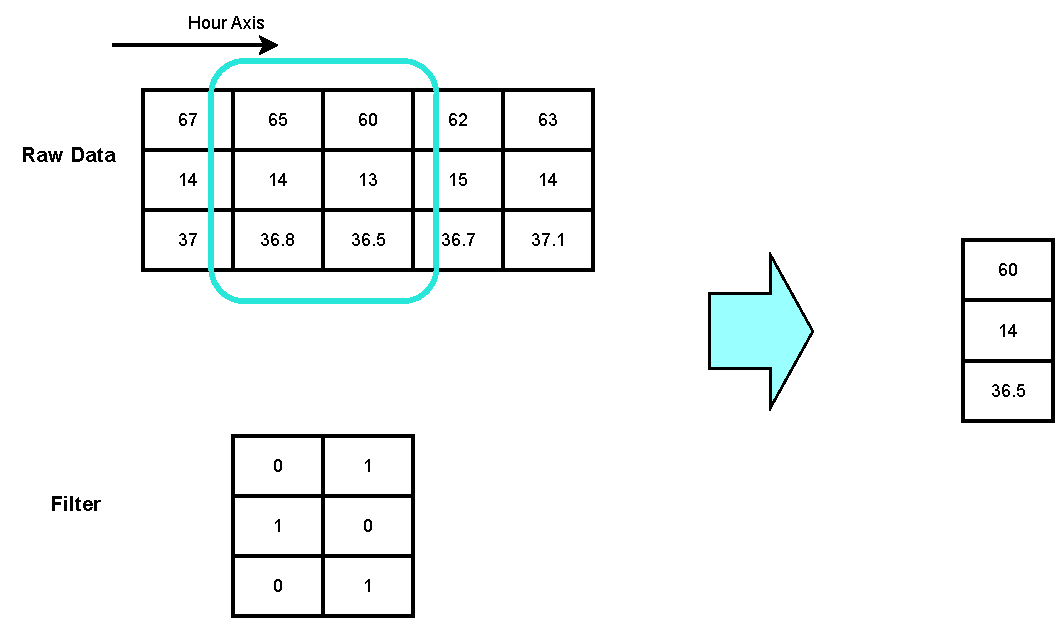
\includegraphics[width=1\textwidth]{thesis/img/convolution.pdf}
  \end{center}
  \caption[Convolution]{An example of Convolution Calculation}
  \label{fig:convolution}
\end{figure*}

Activation function is applied on the new data produced from convolution element-wise to introduce non-linearity into the network as the normal neural network.

Pooling layer is used to reduce the computational complexity and the number of parameters in the neural network, and also prevent overfitting. It is periodically inserted in the CNN. One commonly used technique is MaxPooling where the maximum value within a small window is taken as the output:
\begin{equation}
    \operatorname{MaxPooling}(i, j)=\max \{I(i+m, j+n)\}
\end{equation}
Figure \ref{fig:maxpooling} is an example of MaxPooling

\begin{figure*}
  \begin{center}
    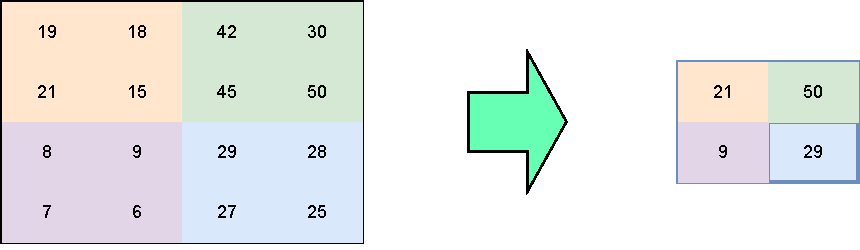
\includegraphics[width=0.8\textwidth]{thesis/img/maxpooling.pdf}
  \end{center}
  \caption[MaxPooling]{An example of MaxPooling}
  \label{fig:maxpooling}
\end{figure*}

Fully connected layer is used after several convolutional and pooling layers to perform the classification or regression task on the learned features, which is flattened into a vector. The output of a fully connected layer is fed into a logistic function, softmax or sigmoid, to obtain class probabilities in classification tasks. As neural network, loss function and backpropgation are also used in CNN to optimize the parameters.


\section{Evaluation}
As aforementioned, , in a regression task, the objective is typically to predict a numerical value as the outcome. The disparity between the actual outcome and the predicted outcome serves as the basis for evaluating the effectiveness of the prediction. Two key metrics are commonly employed for this purpose: Mean Absolute Error (MAE) and Root Mean Square Error (RMSE). Both metrics are widely utilized for assessing the performance of regression models. Here I introduce them, according to \textcite{tyagi2022, chai2014}

Mean Absolute Error (MAE) measures the average absolute difference between the predicted values and the actual values, calculated with: 
\begin{equation}
    \mathrm{MAE}=\frac{1}{n} \sum_{i=1}^n\left|y_i-\hat{y}_i\right|
\end{equation}
where $n$ is the amount of observations, $y_i$ represents the actual value for observation $i$, and $\hat{y}_i$ represents the predicted value for observation $i$. The Mean Absolute Error (MAE) is robust to outliers as it evaluates the absolute differences between actual and predicted values. This metric assigns equal weight to all errors, irrespective of their magnitude. A low MAE signifies small absolute errors between actual and predicted values, indicating higher accuracy. It suggests that the model's predictions closely align with the actual values, without considering the direction of the errors. Conversely, a high MAE indicates poorer performance, characterized by higher prediction errors.

Root Mean Square Error (RMSE) measures the square root of the average of the squared differences between the predicted values and the actual values, calculated with: 
\begin{equation}
    \mathrm{RMSE}=\sqrt{\frac{1}{n} \sum_{i=1}^n\left(y_i-\hat{y}_i\right)^2}
\end{equation}
where $n$ is the amount of observations, $y_i$ represents the actual value for observation $i$, and $\hat{y}_i$ represents the predicted value for observation $i$. Root Mean Square Error (RMSE) penalizes larger errors more heavily than smaller ones due to the squaring operation involved. This sensitivity to outliers arises from this squaring process. A low RMSE indicates that the average magnitude of errors between predicted and actual values is small, signifying that the model's predictions closely match the actual values, indicative of good performance. Conversely, a high RMSE suggests poorer performance.

In addition to these two, another measurement utilized in this study is Mean Square Error (MSE), which is the squared version of RMSE. Like RMSE, MSE also emphasizes larger errors due to its squaring operation, thus sharing similar properties. Its equation can be found in \ref{eq:mse}

Both Mean Absolute Error (MAE) and Root Mean Square Error (RMSE) are measured in the same units as the dependent variable, which is the variable being predicted. Lower values of both metrics indicate better model performance. MAE and RMSE serve as useful metrics for evaluating the accuracy of regression models. MAE demonstrates greater robustness to outliers, while RMSE penalizes larger errors more heavily. 

\section{Explainable Artificial Intelligence}
As previously mentioned, machine learning models are often perceived as "black boxes," as their internal mechanisms can be difficult to interpret, leaving only inputs and outputs observable. In order to enhance the interpretability of these models, this study introduces the concept of SHapley Additive exPlanations (SHAP) values.  

According to \textcite{lundberg2017, camilla_shap}, the SHAP value method aims to elucidate the output of a model by highlighting the contribution of each feature to the model's prediction. Drawing inspiration from cooperative game theory, the concept of SHAP values originates from the Shapley value, which in a coalition game represents each player's fair share of the total payoff.

In the context of machine learning, the input features serve as the "players," while the set of features comprises the "coalition." The disparity between the actual prediction and the average prediction made by the model constitutes the "payoff." SHAP value computation involves assessing the contribution of each feature to the prediction by considering all possible combinations of features and their respective marginal contributions. The kernel SHAP value calculation assumes all the features contribute to the model, and from which I can get the contribution of feature $i$ with:
\begin{equation}
    \phi_i(x)=\sum_{S \subseteq\{1,2, \ldots, M\} \backslash\{i\}} \frac{|S| !(M-|S|-1) !}{M !}\left[f\left(x_{S \cup\{i\}}\right)-f\left(x_S\right)\right]
\end{equation}
where $\phi_i(x)$ is the SHAP value of feature $i$ for instance $x$, $S$ represents a subset of features excluding feature $i$, $M$ is the total number of features, $f(x_S)$  is the model's prediction for instance $x$ using only the features in subset $S$, and $f\left(x_{S \cup\{i\}}\right)$ is the model's prediction for instance $x$ using features in subset $S$ along with feature $i$. A negative SHAP value indicates that the feature contributes negatively to the prediction, while a positive SHAP value indicates a positive contribution. The absolute SHAP value represents the impact. \textcite{aas2020} proposed approaches to improve SHAP value calculation with different conditional probabilities estimation. 

Differ from correlation coefficient, SHAP values consider not only linear and non-linear relationships but also interactions between features, and the context of the model. SHAP values can be applied in feature engineering as well, to identify which features are most influential in making predictions.
 
\chapter{Experiments}
\label{ch:experiment}
Computational experiments are essential for investigating the research inquiries within machine learning. The objective here is to delineate the experiments, elucidate their execution, and present their outcomes. This chapter will introduce two specific experiments, detailing their data preparation, feature engineering, and execution procedures.

In this study, two experiments were conducted. The objective of both experiments is to utilize bedside data from the initial 12 hours, which constitutes a shorter time range compared to the Logistic Organ Dysfunction Score (LODS), for predicting LODS after the first day of stay.

Experiment I employs a single value for each feature within the first 12 hours to train a predictive model using the XGBoost algorithm. This experiment incorporates a feature reduction process aimed at achieving high-performance models with a minimal number of features. Model performance is evaluated using Root Mean Square Error (RMSE) and Mean Absolute Error (MAE). SHAP values are also calculated in this experiment to give interpretability.

Experiment II utilizes vital sign data from each hour of the initial 12 hours, alongside various other bedside data, to predict LODS. It involves feature engineering with a model trained using the Convolutional Neural Network (CNN) algorithm, followed by prediction using a model trained with the XGBoost algorithm. This experiment encompasses two separate model training processes and an adjustment process that combines the outputs of both models to achieve optimal performance. Similar to Experiment I, performance evaluation in Experiment II is based on RMSE and MAE metrics.

Both experiments were conducted using a MacBook Air 2022 equipped with an M2 CPU and 24GB of memory. The XGBoost model training utilized the Python XGBoost Library, while PPCA (Probabilistic Principal Component Analysis) was performed using Matlab as described by \textcite{jakob2015}. The CNN models were implemented using TensorFlow.

\section{Data Collection}
Based on research from \textcite{asuroglu2021, johnson2013}, vital signs and the Glasgow Coma Scale are commonly utilized bedside data in this field of research. In this study, twelve measurements were collected during the initial 12-hour ICU stays, encompassing heart rate, systolic and diastolic blood pressure, mean blood pressure, respiratory rate, temperature, oxygen saturation, urine output, ventilation status, Glasgow Coma Scale, Glasgow Coma Scale eye opening, and Glasgow Coma Scale Motor. The maximum, minimum, and average values of the first seven measurements were recorded for each hour of the initial 12 hours. Additionally, the total urine output over the 12-hour period was collected, along with the most severe value recorded for the remaining parameters during the 12-hour window.

Ventilation status was categorized starting from the most critical condition: tracheostomy, invasive ventilation, non-invasive ventilation, high-flow nasal cannula (HFNC), supplemental oxygen, and none. It is noted that in many instances, when patient data was recorded within the 4 hours preceding ICU admission, no data was recorded for the first hour post-admission. Therefore, data collection for the first hour includes the preceding 4 hours before ICU admission as well as the first hour within the ICU. Moreover, patients' age and gender are also collected, where gender are coded with 0 for Male and 1 for Female.

Three additional inclusion criteria are applied when prepare the dataset: 1) patients are aged over 18, 2) patients stayed in ICU for more than 24 hours so that there is LODS value calculated, 3) for each vital sign, there is at least one measured value in the first 12 hours. As a result, there are 8034 records included in this study, as Figure \ref{fig:include_criteria}.

\begin{figure*}
  \begin{center}
    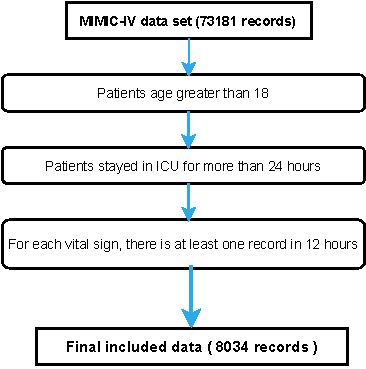
\includegraphics[width=0.8\textwidth]{thesis/img/include_criteria.pdf}
  \end{center}
  \caption[Inclusion Criteria]{Inclusion Data Criteria}
  \label{fig:include_criteria}
\end{figure*}

After applying the inclusion criteria, a total of 8034 records were included in the experiments. The distribution of records for each LODS value can be found in Figure~\ref{fig:lods_distri_fig}
%\ref{table:records_amount_per_lod} 

\begin{figure}[t]
  \begin{center}
    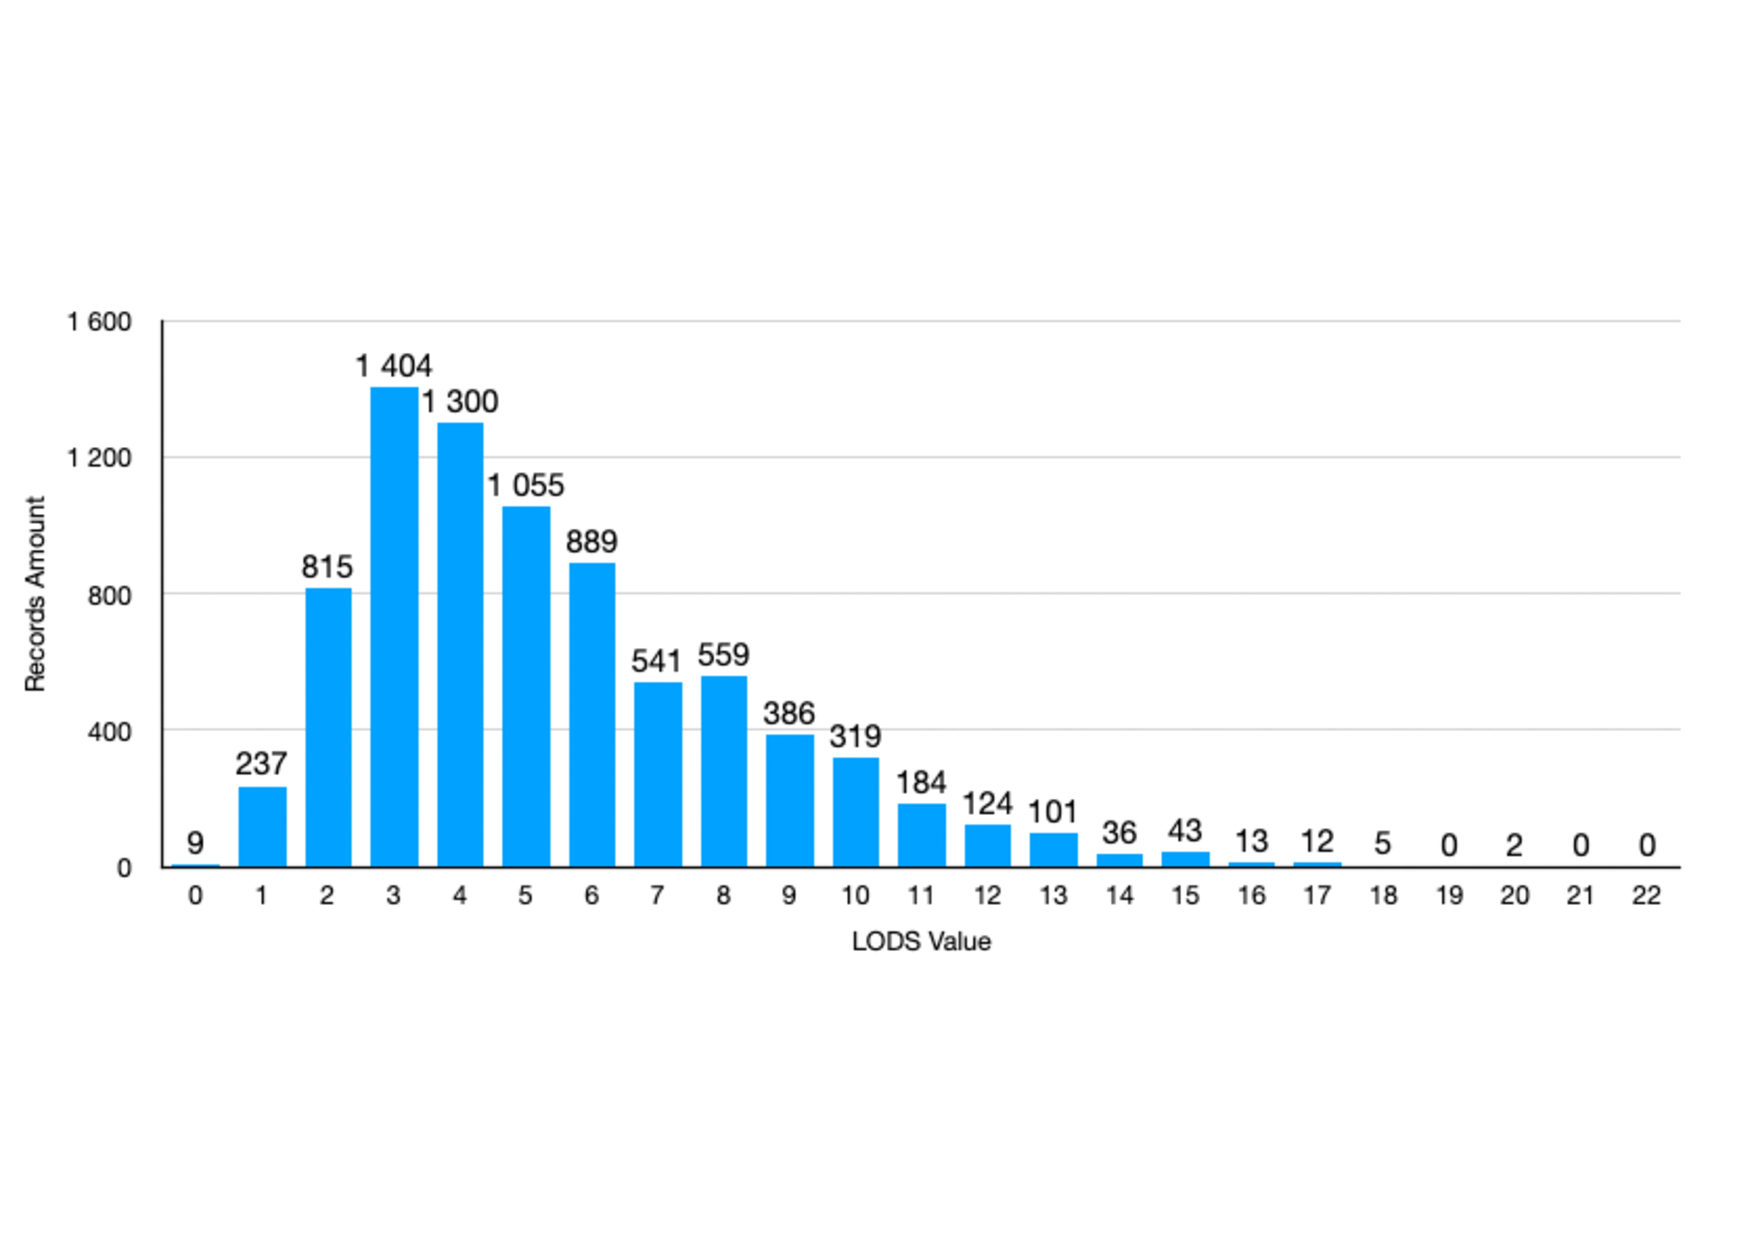
\includegraphics[width=1.0\textwidth]{thesis/img/lods_record_distribution.pdf}
  \end{center}
  \caption[Record amount of each lods value]{Records amount distribution of each LODS value}
  \label{fig:lods_distri_fig}
\end{figure}


\begin{comment}
\begin{table}[]
\centering
    \caption{Records amount per LODS value}
    \label{table:records_amount_per_lod}
    \begin{tabular}{|l|l|}
    \hline
        \textbf{LODS Value} & \textbf{Amount} \\ \hline
        0 & 9 \\ \hline
        1 & 237 \\ \hline
        2 & 815 \\ \hline
        3 & 1404 \\ \hline
        4 & 1300 \\ \hline
        5 & 1055 \\ \hline
        6 & 889 \\ \hline
        7 & 541 \\ \hline
        8 & 559 \\ \hline
        9 & 386 \\ \hline
        10 & 319 \\ \hline
        11 & 184 \\ \hline
        12 & 124 \\ \hline
        13 & 101 \\ \hline
        14 & 36 \\ \hline
        15 & 43 \\ \hline
        16 & 13 \\ \hline
        17 & 12 \\ \hline
        18 & 5 \\ \hline
        19 & 0 \\ \hline
        20 & 2 \\ \hline
        21 & 0 \\ \hline
        22 & 0 \\ \hline
        \textbf{Total:} & 8034 \\ \hline
    \end{tabular}
\end{table}
\end{comment}

\section{Experiment I: Correlation Coefficient and XGBoost}

In Experiment I, our objective is to construct a straightforward yet highly accurate prediction model by leveraging a minimal set of features. To achieve this, I collected the maximum, minimum, and average values of the seven vital signs over the 12-hour period, along with other relevant features.

In this experiment, I employed Pearson Correlation Coefficient and Spearman Correlation Coefficient individually. Consequently, I trained two distinct models for this experiment, comparing their performance using RMSE and MAE metrics. Additionally, I incorporated models trained with alternative algorithms to provide further comparison.

To enhance our understanding of model behavior, I calculated SHAP values to assess the contribution of features within each model. This analysis allows us to gain insights into the relative importance of different features in the predictive process.

During the data collection phase of this study, I rigorously applied criteria 3, which mandated that each vital sign must have at least one recorded measurement within the initial 12 hours of observation. This meticulous criterion ensured that all features included in Experiment I possessed recorded values, effectively eliminating any instances of missing data in our dataset. Moreover, it is worth noting that all recorded values represent real measurements obtained during the observational period. 

\subsection{Feature Reduction}
Upon reviewing the data, I observed instances where certain patients exhibited aberrant maximum and minimum values for a particular vital sign, potentially stemming from recordings taken at different times. However, the average value for these patients fell within the normal range. This discrepancy led us to conclude that relying solely on average values may not accurately reflect the true condition of the patient in this experiment. Consequently, I made the decision to discard the average values from this experiment. 

To streamline the feature set, I chose to gather the worst value for each vital sign, aligning with the guidelines found in LODS and several other scoring systems. To determine the worst value, I introduced a baseline value for each vital sign. This involved calculating the absolute difference between the minimum/maximum value and the baseline value. Subsequently, the worst value was identified as the one exhibiting the larger absolute difference from the baseline value. This approach ensures the inclusion of the most pertinent values for each vital sign.

For adults, the normal range for each vital sign is typically defined by a range of values. To establish a baseline value, I adopted the median of this range, drawing upon references such as \textcite{medlineplus, johnsh, torp2023, yalemed}. The baseline values are detailed in Table \ref{table:baseline_value}. To determine the worst value for each vital sign, I compare the recorded minimum and maximum values against the corresponding baseline value. The value with the larger absolute difference from the baseline is identified as the worst value. For example, if a patient's maximum heart rate is recorded as 101 and the minimum heart rate is 65 within the first 12 hours, then 101 would be considered the worst value for heart rate. This process is applied uniformly across all vital signs.
 
\begin{table}[ht]
\centering
    \caption{Baseline values used in experiment I}
    \label{table:baseline_value}
    \begin{tabular}{|l|l|}
        \hline
        \textbf{Measurements} & \textbf{Baseline Value}\\ \hline
            Heart Rate& 80                \\ \hline
            Systolic Blood Pressure& 120               \\ \hline
            Diastolic Blood Pressure& 80                \\ \hline
            Mean Arterial Pressure& 100               \\ \hline
            Respiratory Rate& 14\\ \hline
            Temperature& 37\\ \hline
            Oxygen Saturation& 98                \\\hline
    \end{tabular}
\end{table}

\subsection{Model Training}

After reducing the features, all collected records were divided into an 80:20 ratio for training and testing purposes, respectively. With a total of 8034 records available, 6427 records were allocated for training the model, while the remaining 1607 records were reserved for testing. During the model training process, which encompasses both training and validation, the testing records were not utilized. These reserved records are exclusively employed for evaluating the model's performance after it has been trained on the training dataset. 

The original intention behind utilizing both Pearson Correlation Coefficient and Spearman Correlation Coefficient was to amalgamate their results to identify the best feature set. However, after applying two correlation coefficients to assess the correlation between LODS values and each parameter, I obtained results as presented in Table \ref{table:cc_value}. Notably, I observed that while the direction of correlation (negative or positive) remained consistent across both coefficients, the actual correlation values and rankings differed. Consequently, I made the decision to train models utilizing both correlation rankings and subsequently compare the results. At this stage, I employed sequential backward selection to identify the optimal feature set. The selection process involved removing features in order of their absolute correlation values, from low to high. Given the high correlation value of 0.7687 between GCS Motor and GCS Eyes in the Pearson correlation, I opted to retain GCS Motor for training the model, as it exhibited a higher correlation value with LODS compared to GCS Eyes, only in the model trained based on Pearson Correlation.

Moreover, I adjusted hyperparameters such as tree amount and tree depth to mitigate the risk of overfitting during model training. This proactive measure ensures that our models generalize well to unseen data and produce reliable predictions.

\begin{table}[ht]
\centering
    \caption{Pearson and Spearman correlation coefficient}
    \label{table:cc_value}
    \begin{tabular}{|l|l|l|}
        \hline
        \textbf{Feature} & \textbf{Pearson} & \textbf{Spearman} \\ \hline
            GCS & -0.4286 & -0.1977 \\ \hline
            GCS Motor & -0.4057 & -0.3932 \\ \hline
            GCS Eyes & -0.3645 & -0.3396 \\ \hline
            Ventilation & -0.2618 & -0.2705 \\ \hline
            SPO2 & -0.2341 & -0.1416 \\ \hline
            Urine Output & -0.2300 & -0.3154 \\ \hline
            Respiratory Rate & 0.1715 & 0.1566\\ \hline
            Heart Rate & 0.1633 & 0.1232 \\ \hline
            sbp & -0.1572 & -0.2479 \\ \hline
            dbp & -0.1109 & -0.2133 \\ \hline
            map & -0.0889 & -0.2780 \\ \hline
            Temperature & -0.0638 & -0.0067 \\ \hline
            Age & 0.0505 & 0.0705 \\ \hline
            Gender & 0.0146 & 0.0121 \\ \hline
    \end{tabular}
\end{table}


\section{Experiment II: Convolutional Neural Network and XGBoost}

According to an interview with a medical doctor, \enquote{When assessing a patient's situation, what clinicians are interested in is the trend of changes in vital signs.} (Personal communication with medical doctor Matti Onnela, Assistant Chief of Cardiology at Heart Hospital Hämeenlinna, Licensiate of Medicine, at [Aug 21, 2023]). The target of Experiment II is using data of each hour in the first 12 hours to predict LODS so that I can take vital signs trend analysis as part of the features for prediction.

In this experiment, I collected the maximum, minimum, and average values of vital signs for each hour within the initial 12-hour period, including heart rate, systolic blood pressure (sbp), mean arterial pressure (map), diastolic blood pressure (dbp), oxygen saturation (spo2), temperature, and respiratory rate. Additionally, I incorporated total urine output, worst ventilation status, and worst Glasgow Coma Scale (GCS) values recorded during the first 12 hours.

Due to differences in patients' physical conditions, the focus of life monitoring varies, leading to different patterns of data missing. When observing the data of an individual patient, the frequency of collecting different vital signs varies. Similarly, when observing the same vital sign across all patients, there can be significant differences in the frequency of data collection. These missing data points are primarily categorized as missing at random (MAR). And there are also some data missing completely at random (MCAR) as it is the only missing value of all vital signs in the whole 12 hours.

To address the missing data, I employed two separate imputation methods: Linear Interpolation and Probabilistic Principal Component Analysis (PPCA). Subsequently, models were trained using the datasets imputed with each method individually. Performance comparison was conducted using Mean Absolute Error (MAE) and Root Mean Square Error (RMSE) metrics.

\subsection{Missing Data Imputation}

In this experiment, two missing data imputation methods, namely linear interpolation and Probabilistic Principal Component Analysis (PPCA), were applied. The missing data occurred exclusively in the vital signs data, which should ideally consist of 21 values per hour for each of the 12 hours.

To facilitate the imputation process, the available data were structured in a 21x12 matrix, ordered chronologically according to time-series. This matrix format allowed for a systematic approach to missing data imputation, enabling the application of both linear interpolation and PPCA methods effectively.

When imputing missing data, our aim is to maintain the overall trend of the data. For this purpose, I apply linear interpolation to calculate missing values. Specifically, if data for the first hour or the first several hours are missing, I propagate the first recorded data value across those missing hours. Similarly, if data for the last hour or the last several hours are missing, I extend the last recorded data value to cover those missing hours. This approach ensures consistency and coherence in the imputed dataset while preserving the temporal trends observed in the original data.

In the PPCA process, each record undergoes its own missing data imputation procedure, as the criteria for missing data varies from record to record. This individualized imputation is carried out using probabilistic calculations, with PPCA executed using MATLAB. Since the imputation involves probability calculations, different values may be imputed for the same missing data in different PPCA runs. To mitigate this variability, the imputation process is repeated five times.

To assess the quality of the imputed values, I randomly select 10 values from each imputation run and compare them. The criterion for selecting the better-imputed value is based on proximity to the average of the values observed five hours before and after the missing value. The three files with the most "better-imputed results" are randomly combined to create a new dataset for training purposes. This approach ensures that the imputed dataset reflects the most reliable imputed values, contributing to the robustness of the subsequent model training process.


\subsection{Feature Engineering}

In this experiment, the processing of vital signs differs from that of other variables due to their distinct nature. Vital signs are collected on an hourly basis and undergo feature engineering to extract features from the 21x12 data matrix. This approach is chosen because vital signs are typically recorded hourly, resulting in a dense time-series dataset. Feature engineering enables us to extract meaningful features from this dense data, capturing relevant patterns and trends. On the other hand, variables include total urine output, ventilation status, and GCS values, are processed differently because 1) rine output might not be an continuous operation happens in every hour or not recorded as frequent as vital signs. 2) GCS values are often recorded infrequently, with fewer than three recordings typically observed within the first 12 hours. Thus, the raw values are utilized directly in the analysis. 3) Ventilation status tends to change minimally over time. Therefore, feature engineering is unnecessary, and the raw ventilation status data are used directly in the analysis.

After reviewing the imputed missing data, I have decided to retain only the average value for several reasons: 1) Patients' physiological parameters typically do not undergo large changes within a single hour. Consequently, the difference between the maximum and minimum values within an hour is typically negligible. Therefore, there is no substantial benefit to performing a worst-case check, as was done in Experiment I. 2) In most cases, only one value is recorded for each vital sign per hour. This means that the maximum, minimum, and average values are identical. 3) Maintaining consistency in the data trend is crucial. When considering trends, it is either all values are maximum or all values are minimum within an hour. However, if the worst value fluctuates between maximum and minimum, it can disrupt the trend analysis. On the other hand, the average value effectively captures the trend without the potential for such disruption. 

In this experiment, the Convolutional Neural Network (CNN) algorithm is applied to the remaining 7x12 data (after feature extraction from the vital signs data). The goal is to extract features from this data. To train the CNN models, two datasets are utilized: one imputed with linear interpolation and the other with PPCA. The target variable is set as the LODS, while the average vital signs of the first 12 hours serve as the input features.

Separate CNN models are trained for each dataset, and their performance is evaluated using Mean Squared Error (MSE) and Mean Absolute Error (MAE). The best-performing model from each dataset is selected to extract the features. To extract features, the last layer of each CNN model is removed, and the output from the previous layer is retained. These outputs serve as the features for further analysis or model training tasks. This approach allows for the creation of meaningful and informative features derived from the input data. MAE and MSE of two models can be found in Table \ref{table:cnn_result_comparison}

\begin{table}[ht]
\centering
    \caption{Feature engineering with CNN result comparison}
    \label{table:cnn_result_comparison}
    \begin{tabular}{|l|l|l|}
        \hline
        \textbf{Imputation Method} & \textbf{MAE} & \textbf{MSE} \\ \hline
        Linear Interpolation & 2.0494 & 6.9286 \\ \hline
        PPCA & 2.0503 & 6.8565 \\ \hline
    \end{tabular}
\end{table}

\subsection{Model Training}

In the model training phase, the features extracted from the CNN algorithm are combined with other relevant features, including total urine output, the worst ventilation status, and the worst Glasgow Coma Scale (GCS) related values. However, gender and age are excluded from this experiment due to their low correlation coefficients, as indicated in Table \ref{table:cc_value} from Experiment I. This decision is based on the understanding that features with low correlation coefficients may have limited predictive power and may not significantly contribute to the model's performance. Therefore, removing gender and age helps streamline the feature set.

Indeed, managing the number of features is crucial for optimizing the performance of XGBoost model. However, in CNN model, the parameter of the last layer decides the amount of outputted values. To achieve optimal performance, it is essential to adjust both models in tandem. In the CNN model, parameters are adjusted from the last layer towards the first layer, primarily focusing on the output amount. This adjustment ensures that the CNN model outputs an appropriate number of features that can effectively complement the XGBoost model.

On the other hand, in the XGBoost model, the number of trees and the maximum depth of each tree are adjusted to balance the number of input features from the CNN model. This balancing act aims to prevent overfitting and maximize the performance of the combined model. By fine-tuning both models simultaneously, I can ensure that the features extracted from the CNN model are effectively utilized by the XGBoost model, resulting in improved predictive performance while mitigating the risk of overfitting.

\chapter{Results}
\label{ch:results}
This chapter presents the results of the two experiment, encompassing the models' structure, performance of models in both experiments, and explanation result in experiment I.

\section{Experiment I: Correlation Coefficient and XGBoost}

As a result of Experiment I, I have developed two models based on different correlation methods: XG-Pearson and XG-Spearman.

XG-Pearson model comprises 8 features: GCS, GCS Motors, Ventilation Status, SPO2, Urine output, Respiratory Rate, Heart Rate, and sbp. It achieved the best performance metrics in the test dataset, with an MAE of 1.4173 and RMSE of 1.8222.

On the other hand, XG-Spearman model includes 11 features: GCS, GCS Motors, Ventilation Status, urine output, sbp, mbp, respiratory rate, SPO2, heart rate, GCS Eyes, and dbp. It yielded an MAE of 1.427 and RMSE of 1.840.

Table \ref{table:Perfomance_comparison} presents a performance comparison between the two models and other algorithms. Since there is a lack of research on predicting LODS, I trained models using other algorithms as well for comparison. Both XGBoost models demonstrated superior performance compared to the other models, with the XG-Pearson model slightly surpassing the XG-Spearman model in performance metrics. The XG-Pearson model also has the added advantage of requiring the fewest features.

\begin{table}[ht]
\centering
    \caption{Performance comparison in Experiment I}
    \label{table:Perfomance_comparison}
    \begin{tabular}{|l|l|l|l|l|}
        \hline
        \textbf{Model} & \textbf{Correlation} & \textbf{Features} & \textbf{MAE} & \textbf{RMSE} \\ \hline
        \multirow{2}{*}{Linear Regression} & Spearman & 12 & 1.746 & 2.214 \\ \cline{2-5} 
         & Pearson & 13 & 1.742 & 2.207 \\ \hline
        \multirow{2}{*}{Random Forest} & Spearman & 14 & 1.434 & 1.856 \\ \cline{2-5} 
         & Pearson & 13 & 1.433 & 1.856 \\ \hline
        \multirow{2}{*}{XGBoost} & Spearman & 11& 1.427& 1.840\\ \cline{2-5} 
         & \textbf{Pearson} & \textbf{8} & \textbf{1.417} & \textbf{1.822} \\ \hline
    \end{tabular}
\end{table}

Figure \ref{fig:experiment_1_result} illustrates the comparison of results between the two models. In the Actual vs. Predicted plots, shown in subfigures \ref{subfig:xg_pearson} and \ref{subfig:xg_spearman}, the black lines represent the ideal scenario where the predicted value equals the actual value, while the points represent the predicted values plotted against the actual values. These points are marked with varying transparency levels, indicating the density of points in each region. Darker areas indicate higher point density.

From the figure, it is evident that both models perform admirably within the LODS range of 2-5, exhibiting similar distributions. However, within the LODS range of 10-20, the XG-Pearson model demonstrates a superior distribution compared to the XG-Spearman model. This is evidenced by the predicted values of the XG-Pearson model being closer to the black line, indicating better alignment with the actual values in this LODS range.

In the residual plots, depicted in Figure \ref{subfig:xg_pearson_residual} and Figure \ref{subfig:xg_spearman_residual}, the grey lines represent the ideal scenario where there is no difference between the actual value and the predicted value. The points on the plot represent the residual values plotted against the actual values.

Upon analysis of the figures, it is observed that within the LODS range of 2-5, both models perform comparably. The residual plot for XG-Spearman exhibits a slightly wider dispersion of points compared to XG-Pearson, although the residuals are slightly closer to the ideal line. Conversely, within the LODS range of 10-20, the performance trends shift. In this range, the residual plot for XG-Pearson shows residuals that are slightly closer to the ideal line compared to XG-Spearman. However, it is worth noting that the overall residual patterns for both models are similar. Overall, while there are slight variations in performance between the two models across different LODS ranges, their overall residual patterns remain similar.

In the Bland-Altman plots depicted in Figure \ref{subfig:xg_pearson_ba} and Figure \ref{subfig:xg_spearman_ba}, the grey line near 0 represents the mean difference between the predicted and actual values. The other two lines represent the limits of agreement, calculated as the mean difference plus or minus 1.96 times the standard deviation of the differences.

Upon analysis of the figures, it is observed that both models perform well within the LODS range of 0-6, as indicated by their good agreement with the actual values. However, within the LODS range of 7-10, the performance of both models deteriorates. The agreement between the predicted and actual values becomes less consistent, indicating poorer performance in this range. Within the LODS range of 11-22, there are fewer examples available for analysis, limiting the ability to provide a precise assessment of model performance in this range.


\begin{figure*}
  \begin{center}
    \subfigure[XG-Pearson: Actual vs Predicted]{
      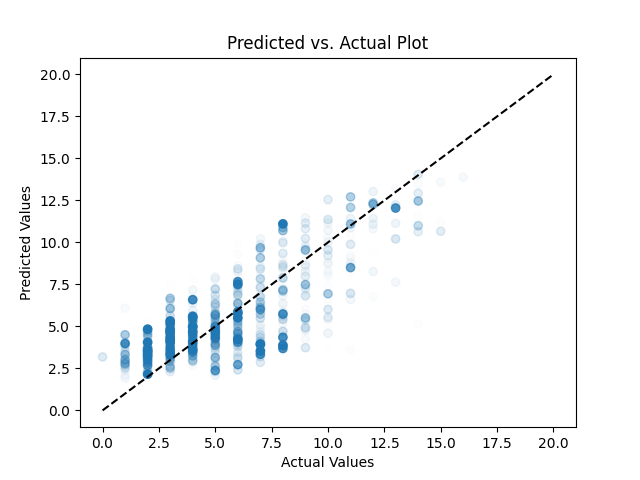
\includegraphics[width=0.45\textwidth]{thesis/img/xg_pearson.png}
      \label{subfig:xg_pearson}}
    \qquad                        
    \subfigure[XG-Spearman: Actual vs Predicted]{
      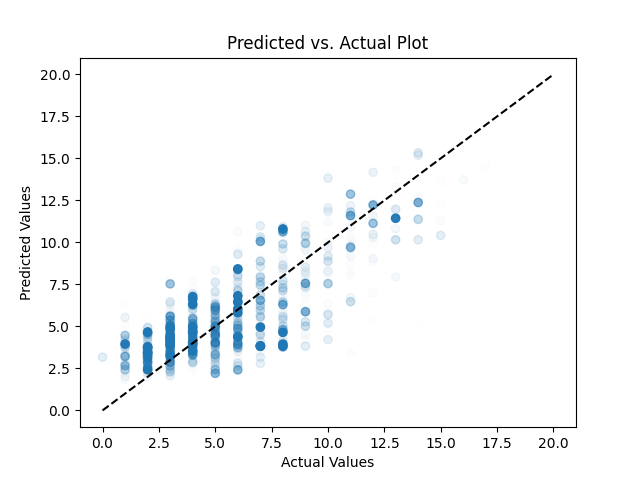
\includegraphics[width=0.45\textwidth]{thesis/img/xg_spearman.png}
      \label{subfig:xg_spearman}}

    \subfigure[XG-Pearson: Residual Plot]{
      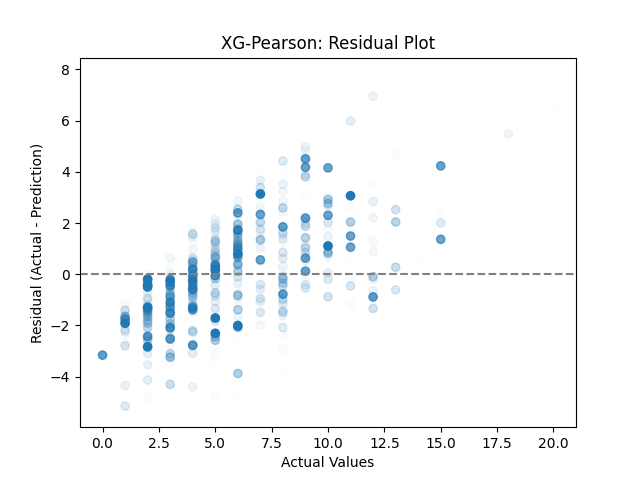
\includegraphics[width=0.45\textwidth]{thesis/img/pearson_residual.png}
      \label{subfig:xg_pearson_residual}}
    \qquad                        
    \subfigure[XG-Spearman: Residual Plot]{
      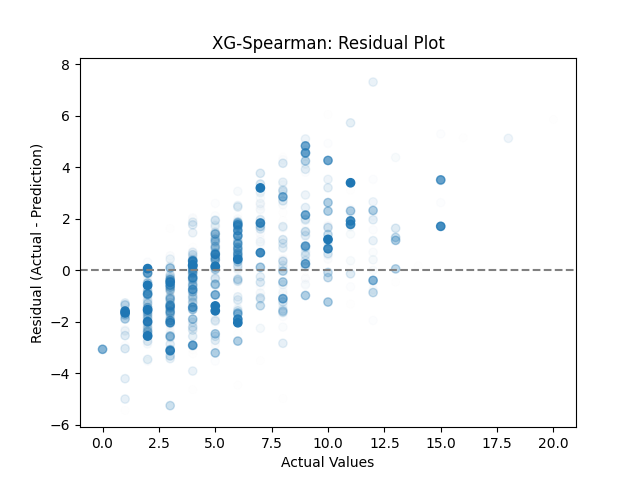
\includegraphics[width=0.45\textwidth]{thesis/img/spearman_residual.png}
      \label{subfig:xg_spearman_residual}}

    \subfigure[XG-Pearson: Bland-Altman]{
      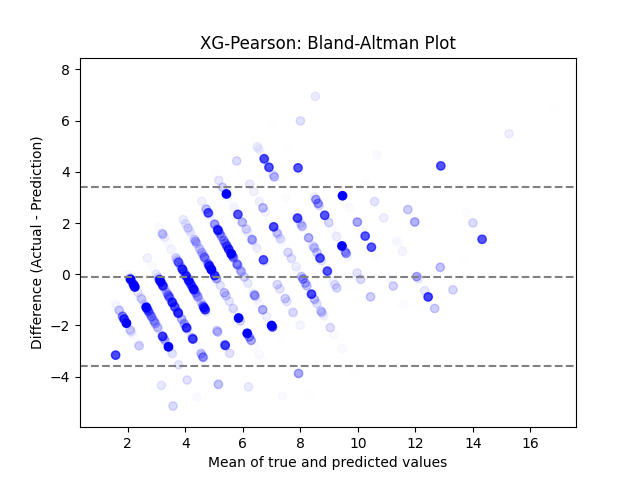
\includegraphics[width=0.45\textwidth]{thesis/img/pearson_ba.png}
      \label{subfig:xg_pearson_ba}}
    \qquad                        
    \subfigure[XG-Spearman: Bland-Altman]{
      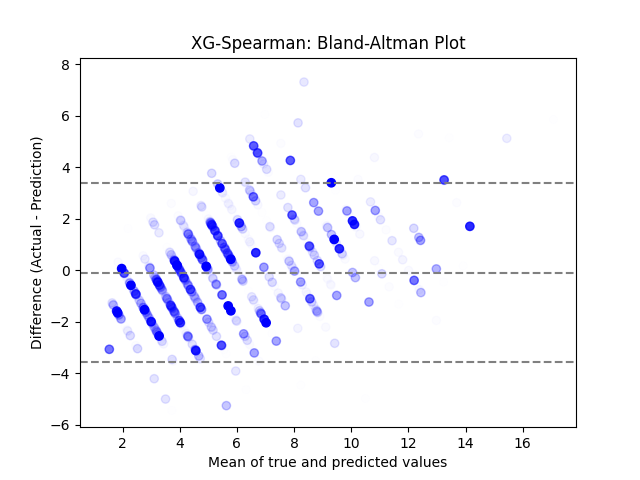
\includegraphics[width=0.45\textwidth]{thesis/img/spearman_ba.png}
      \label{subfig:xg_spearman_ba}}
      
    \caption[Results comparison in Experiment I]{Comparison between models in Experiment I: XG-Pearson and XG-Spearman (The darkness of each point's color is determined by the number of points within each predicted value area of the model. In essence, it reflects the density or concentration of data points within specific ranges of predicted values. Darker colors signify a higher density of data points within those predicted value areas, while lighter colors indicate fewer data points.)}    
    \label{fig:experiment_1_result}
  \end{center}
\end{figure*}


\subsection{Explanation}


In Experiment I, I calculated SHAP values, as depicted in Figure \ref{fig:experiment_1_shap}, to assess the contribution of each feature in the models. From Figure \ref{subfig:xg_pearson_shap}, several insights can be gleaned:
\begin{itemize}
\item Total urine output exhibits a high contribution, both with high and low values. This could be attributed to urine output directly reflecting renal function, an organ covered in LODS scoring.
\item Glasgow Coma Scale (GCS) values show varying contributions. Low GCS values indicate higher danger and contribute significantly, whereas high GCS values contribute less or may even have a negative impact. This suggests that when patients' neurological status is stable, the model relies more on other features. 
Similar trends are observed with GCS Motor, indicating neurological status.
\item Heart rate and sbp, which may indicate cardiovascular status, show significant contributions regardless of whether they are high or low.
\item Ventilation status and respiratory rate, representing pulmonary status, exhibit notable contributions. Interestingly, both high and low respiratory rates contribute significantly, while the contribution from low ventilation status (highly mechanical ventilation) is comparatively lower. This discrepancy may be influenced by the limited number of examples with highly mechanical ventilation status in the dataset.
\item Spo2, indicating hematologic status, primarily contributes when SPO2 levels are low. The maximum limit value of SPO2 also serves as an indicator of normality, with only low values contributing significantly to the prediction.
\end{itemize}

When examining the XG-Spearman model, it is observed that the features shared with XG-Pearson exhibit similar trends but with slight differences in contribution values. However, for the other features:
\begin{itemize}
\item GCS Eyes shows consistently low contribution values regardless of whether the values are high or low.
\item DBP and MBP, which also indicate cardiovascular status, exhibit different contribution patterns. Low MBP contributes significantly in a positive way and slightly in a negative way, while high MBP contributes negatively. Conversely, DBP works in the opposite manner.
\end{itemize}

Overall, the SHAP values provide valuable insights into the contributions of different features to the model predictions, shedding light on the factors influencing LODS scoring. These differences in contribution patterns highlight the nuances in how each feature influences the predictions of the XG-Spearman model compared to the XG-Pearson model. Despite some similarities in trends, the specific contributions of certain features can vary between the two models.


\begin{figure*}
  \begin{center}
    \subfigure[XG-Pearson: SHAP values]{
      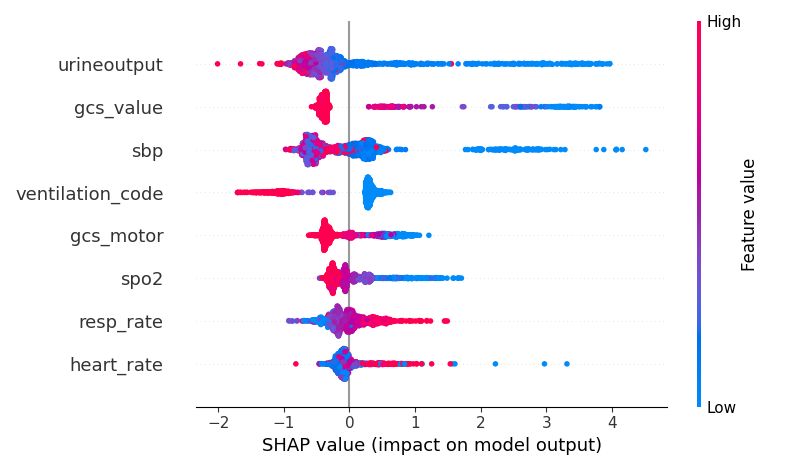
\includegraphics[width=0.45\textwidth]{thesis/img/pearson_shap.png}
      \label{subfig:xg_pearson_shap}}
    \qquad                        
    \subfigure[XG-Spearman: SHAP values]{
      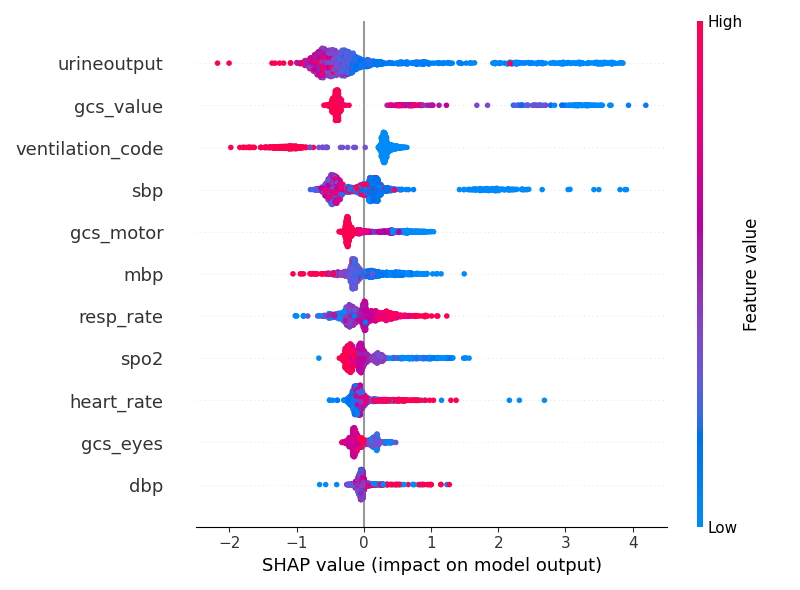
\includegraphics[width=0.45\textwidth]{thesis/img/spearman_shap.png}
      \label{subfig:xg_spearman_shap}}
    \caption[SHAP values in Experiment I]{SHAP Values Plot in Experiment I: XG-Pearson and XG-Spearman}    
    \label{fig:experiment_1_shap}
  \end{center}
\end{figure*}


\section{Experiment II: Convolutional Neural Network and XGBoost}

After fine-tuning, I developed two models in Experiment II. Figure \ref{fig:xg_cnn_li_struc} illustrates the details of the model trained with XGBoost-CNN-Linear Interpolation (Hereinafter referred to as XG-CNN-LI), while Figure \ref{fig:xg_cnn_ppca_struc} depicts the details of the model trained with XGBoost-CNN-PPCA (Hereinafter referred to as XG-CNN-PPCA). These models have different layer parameters, reflecting the distinct configurations optimized for each method of data imputation.

\begin{figure*}
  \begin{center}
    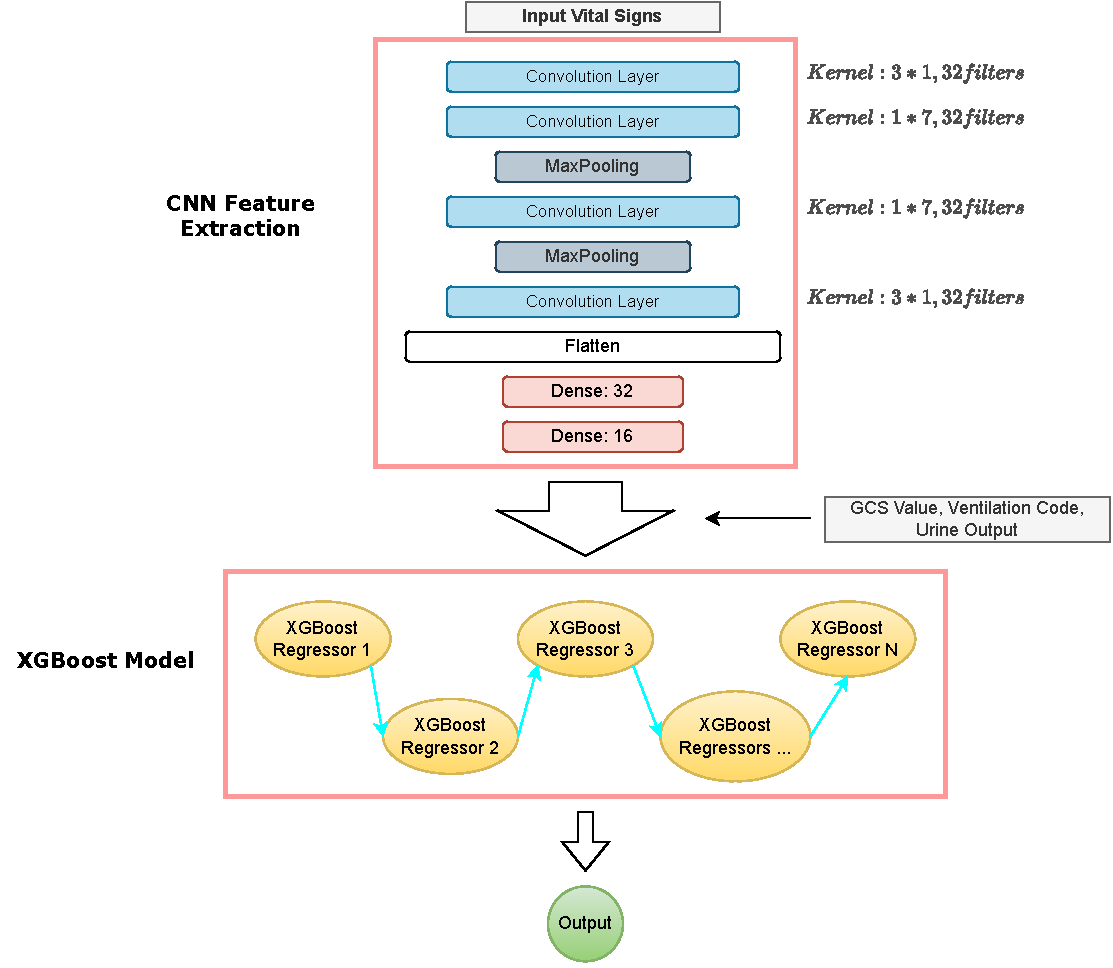
\includegraphics[width=1\textwidth]{thesis/img/xg_cnn_li.pdf}
  \end{center}
  \caption[XGBoost-CNN-LI model]{Model structure of XGBoost-CNN-Linear Interpolation}
  \label{fig:xg_cnn_li_struc}
\end{figure*}

\begin{figure*}
  \begin{center}
    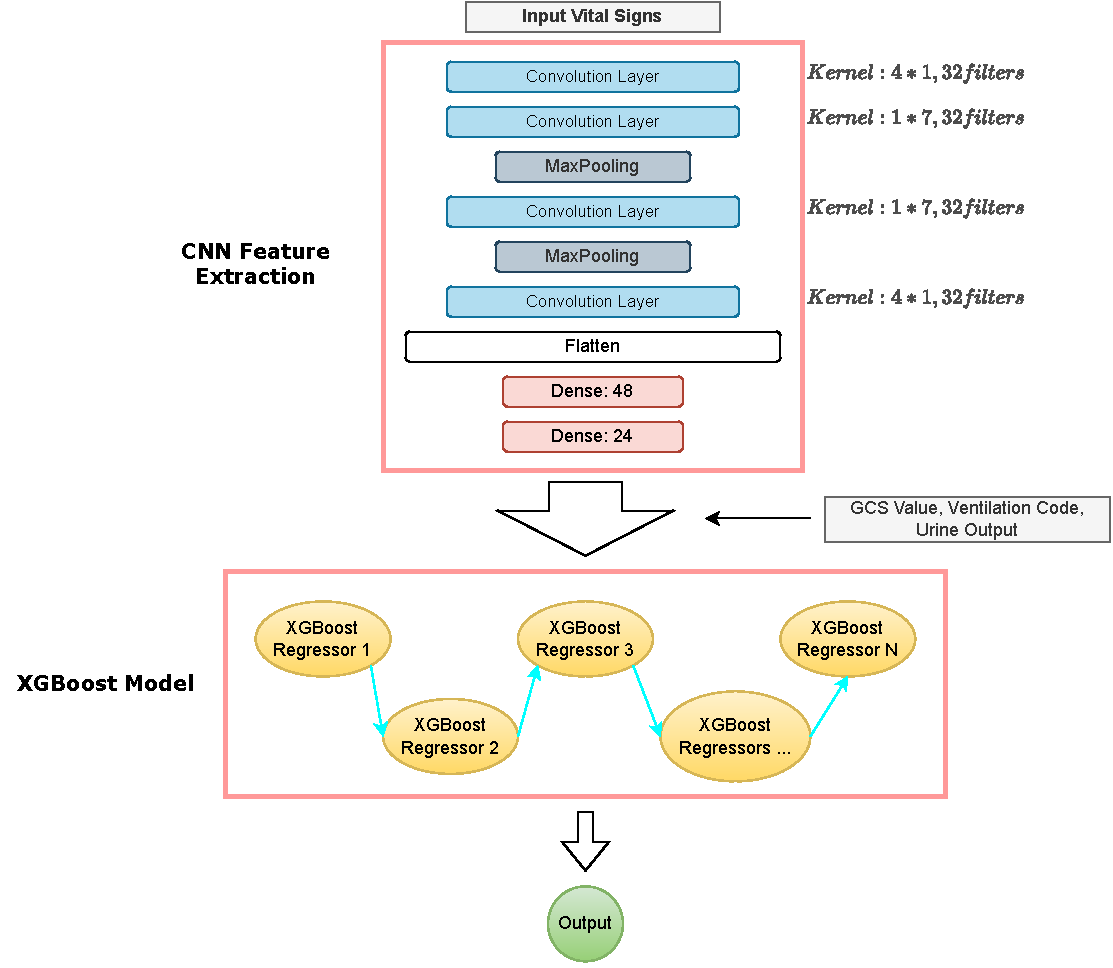
\includegraphics[width=1\textwidth]{thesis/img/xg_cnn_ppca.pdf}
  \end{center}
  \caption[XGBoost-CNN-PPCA model]{Model structure of XGBoost-CNN-PPCA}
  \label{fig:xg_cnn_ppca_struc}
\end{figure*}
As a result, with XG-CNN-LI, I obtained a model that combines a CNN model consisting of 9 layers and 16 outputs, along with an XGBoost model with 100 trees. The performance metrics for this model indicate an RMSE of 1.912 and an MAE of 1.481.

Similarly, with XG-CNN-PPCA, I obtained a model that merges a CNN model comprising 9 layers and 24 outputs with an XGBoost model featuring 100 trees. The performance metrics for this model show an RMSE of 1.916 and an MAE of 1.468.

In Figure \ref{fig:experiment_2_result}, the performance comparison of XG-CNN-LI and XG-CNN-PPCA is presented. From the Actual vs Predicted plots (\ref{subfig:xg_cnn_li} and \ref{subfig:xg_cnn_ppca}), where the black lines refer to the perfect situation, several observations can be made. Within the LODS range of 2-5, the points corresponding to XG-CNN-PPCA are closer to the ideal scenario compared to XG-CNN-LI, indicating a better alignment between predicted and actual values in this range. However, within the LODS range of 6-15, the points for XG-CNN-PPCA appear slightly more dispersed compared to XG-CNN-LI. This suggests that there may be greater variability in the predicted values of XG-CNN-PPCA within this range. This also explains why XG-CNN-PPCA has higher RMSE. Overall, XG-CNN-PPCA performs closer to the ideal scenario across the entire LODS range compared to XG-CNN-LI, indicating superior predictive accuracy and consistency.

In the residual plots (\ref{subfig:xg_cnn_li_residual} and \ref{subfig:xg_cnn_ppca_residual}), where the grey line represents the ideal scenario, several observations can be made. Residuals of XG-CNN-PPCA are generally closer to the ideal line compared to XG-CNN-LI, particularly within the LODS range of 2-5. This suggests that XG-CNN-PPCA exhibits better alignment between predicted and actual values within this range. However, within LODS ranges over 6, both models demonstrate similar residual patterns, indicating comparable performance in these ranges. Notably, in the residual plot of XG-CNN-PPCA, there are more points with larger residuals compared to XG-CNN-LI, particularly evident when LODS is 4. This indicates that XG-CNN-PPCA may have a higher degree of variability or error in predictions for certain LODS values compared to XG-CNN-LI.


Upon analyzing the Bland-Altman plots (\ref{subfig:xg_cnn_li_ba} and \ref{subfig:xg_cnn_ppca_ba}), where the grey line near 0 represents the mean difference and the other two lines represent the limits of agreement, several observations can be made. Within the LODS range of 0-5, both XG-CNN-LI and XG-CNN-PPCA demonstrate good agreement with the actual values, as indicated by the points being clustered around the mean difference line and falling within the limits of agreement. Within the LODS range of 6-12, XG-CNN-PPCA shows slightly better agreement with the actual values compared to XG-CNN-LI. This is evident from the points being more tightly clustered around the mean difference line and falling within narrower limits of agreement. Overall, XG-CNN-PPCA exhibits better agreement with the actual values across all LODS ranges compared to XG-CNN-LI, indicating superior performance in terms of predictive accuracy and consistency.


\begin{figure*}
  \begin{center}
    \subfigure[XG-CNN-LI: Actual vs Predicted]{
      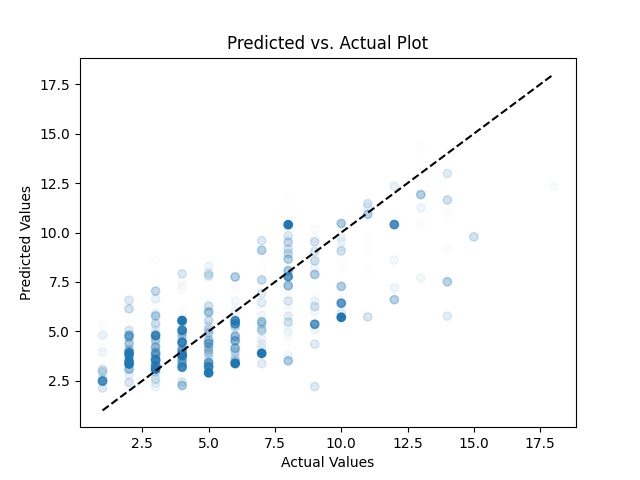
\includegraphics[width=0.45\textwidth]{thesis/img/xg_cnn_li.png}
      \label{subfig:xg_cnn_li}}
    \qquad                        
    \subfigure[XG-CNN-PPCA: Actual vs Predicted]{
      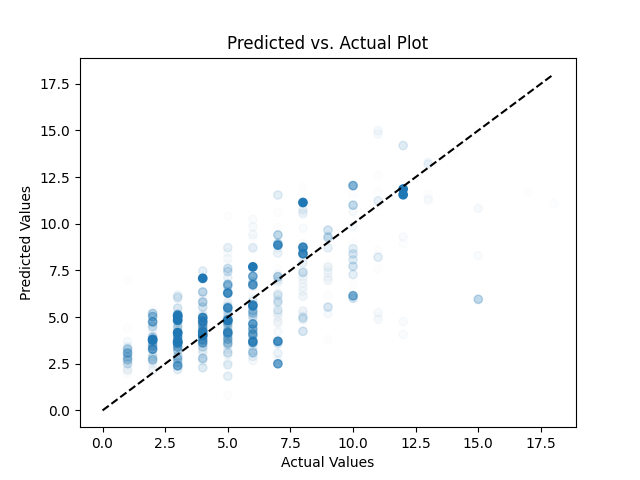
\includegraphics[width=0.45\textwidth]{thesis/img/xg_cnn_ppca.png}
      \label{subfig:xg_cnn_ppca}}

    \subfigure[XG-CNN-LI: Residual Plot]{
      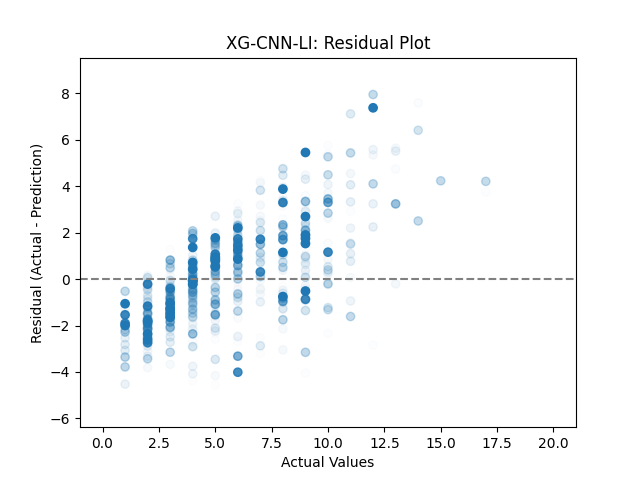
\includegraphics[width=0.45\textwidth]{thesis/img/li_residual.png}
      \label{subfig:xg_cnn_li_residual}}
    \qquad                        
    \subfigure[XG-CNN-PPCA: Residual Plot]{
      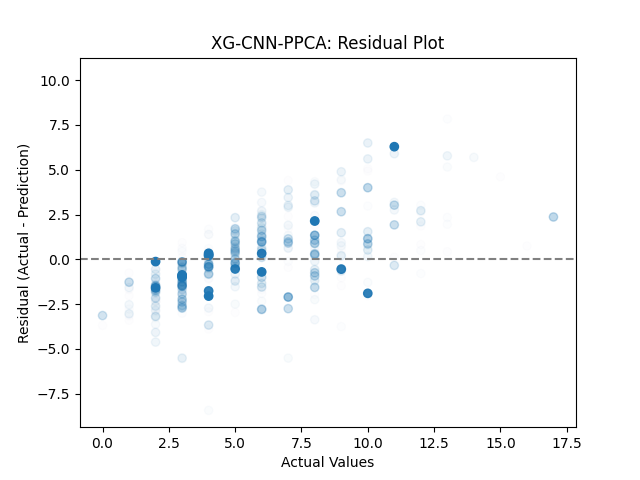
\includegraphics[width=0.45\textwidth]{thesis/img/ppca_residual.png}
      \label{subfig:xg_cnn_ppca_residual}}

    \subfigure[XG-CNN-LI: Bland-Altman]{
      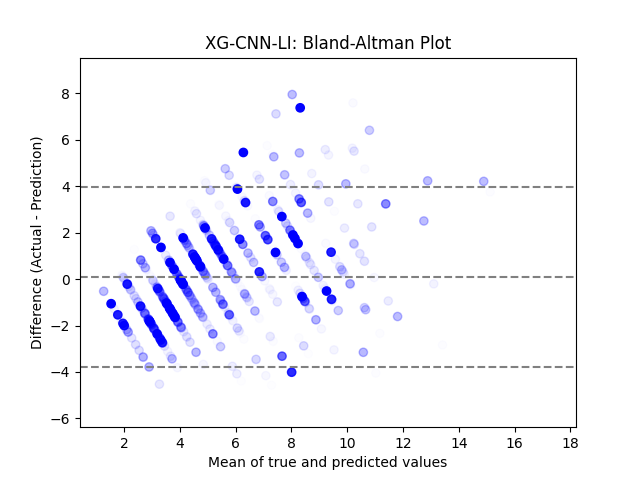
\includegraphics[width=0.45\textwidth]{thesis/img/li_ba.png}
      \label{subfig:xg_cnn_li_ba}}
    \qquad                        
    \subfigure[XG-CNN-PPCA: Bland-Altman]{
      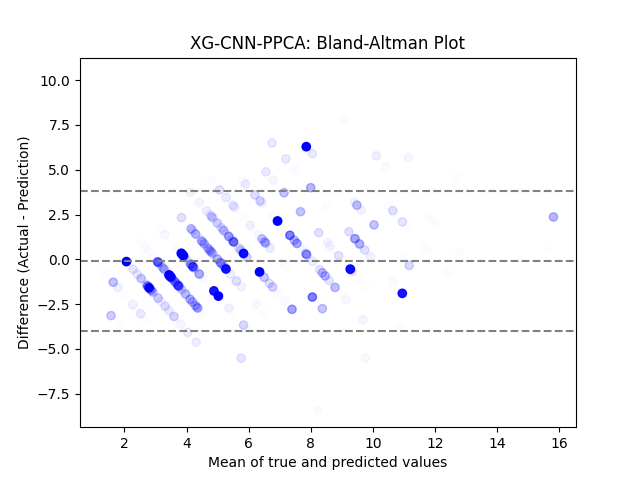
\includegraphics[width=0.45\textwidth]{thesis/img/ppca_ba.png}
      \label{subfig:xg_cnn_ppca_ba}}
      
    \caption[Results comparison in Experiment I]{Comparison between models in Experiment I: XG-CNN-LI and XG-CNN-PPCA (The darkness of each point's color is determined by the number of points within each predicted value area of the model. In essence, it reflects the density or concentration of data points within specific ranges of predicted values. Darker colors signify a higher density of data points within those predicted value areas, while lighter colors indicate fewer data points.)}
    \label{fig:experiment_2_result}
  \end{center}
\end{figure*}

\chapter{Discussion}
\label{ch:discussion}

In this study, our primary focus lied in predicting the LODS value using bedside data collected within the first 12 hours of ICU admission. The LODS value holds significant clinical relevance as it can be utilized to calculate the probability of mortality. Early prediction of LODS can provide valuable support to healthcare professionals in adjusting treatment plans promptly, thereby potentially improving patient outcomes.

A key objective of our research was to minimize the number of features utilized in the prediction model. By doing so, I aimed to enhance the practicality and ease of clinical application of LODS. These streamlined approaches not only simplified the predictive process but also reduced the complexity associated with interpreting and utilizing the model in real-world clinical settings.

In Experiment I, the XG-Pearson model demonstrated acceptable performance with an MAE of 1.417 and RMSE of 1.822, outperforming other models. Notably, this model succeeded in achieving its objective of utilizing a minimal number of features, employing only 8 features. Considering the MAE of 1.417 within the total LODS range of 22, it represents a relatively small error.

When evaluating the impact of this error on the calculation of mortality probability, it is important to note the significance of LODS ranges. Figure ~\ref{fig:lods_mortality} illustrates that for LODS values within the range of 0-5 and 13-22, the MAE of 1.417 may not significantly affect the mortality probability calculation. However, it becomes more consequential for LODS values falling within the range of 6-12. In this range, even small deviations in LODS can lead to considerable variations in mortality probability. Therefore, while the XG-Pearson model demonstrates promising performance overall, it is essential to consider the potential implications of its predictive accuracy, particularly in critical LODS ranges. 

Based on Figure ~\ref{fig:lods_distri_fig}, the majority of records in this study fall within the LODS range of 2-6, accounting for approximately 68\% of all records. Given this distribution, it is crucial to evaluate the performance of the XG-Pearson model within this predominant LODS range.

Referring to Figure ~\ref{fig:experiment_1_result}, which showcases the model's performance, particularly within the LODS range of 2-6, I observe that both XG-Pearson and XG-Spearman models exhibit strong performance. The residuals are minimal and concentrated around 0, indicating a close alignment between the predicted and actual values. This suggests that within the prevalent LODS range of 2-6, both models demonstrate robust predictive capabilities and effectively capture the underlying patterns in the data. However, XG-Pearson has better concentration and similar residual than XG-Spearman.

In Experiment I, both Pearson Correlation Coefficient and Spearman Correlation Coefficient were utilized to assess the relationship between features and the LODS value. Surprisingly, despite the assumption that Pearson Correlation Coefficient, which traditionally measures linear relationships, might not be suitable for assessing the connection between vital signs or ventilation status and LODS values, it yielded more helpful insights compared to Spearman Correlation Coefficient.

Traditionally, Pearson correlation assesses linear relationships between two variables. However, vital signs and ventilation status aren't expected to exhibit a direct linear relationship with LODS values. While some vital signs like heart rate may be involved in LODS parameters, the relationship isn't strictly linear. Nevertheless, this experiment unveils a novel perspective: even when the features and target don't conform to a linear relationship, Pearson Correlation Coefficient can still provide valuable insights into their correlation. This highlights the adaptability and potential utility of traditional statistical measures in unconventional contexts.

Indeed, the SHAP values derived from both the XG-Pearson and XG-Spearman models highlight the significant contributions of certain features, notably urine output, GCS values, heart rate, and systolic blood pressure (sbp). These features are closely associated with the renal, neurologic, and cardiovascular systems, respectively, which are the three organ systems with a maximum LODS score of 5 in the LODS system. Consequently, their heightened contribution to the prediction models can be attributed to their direct relevance to the organ dysfunction being assessed by the LODS score. This underscores the importance of these physiological parameters in predicting and assessing the severity of organ dysfunction in critically ill patients. 

In Experiment II, both the XG-CNN-LI and XG-CNN-PPCA models demonstrated comparable performance, achieving similar levels of accuracy as measured by MSE and RMSE. Overall, both models met the objectives of the study, indicating their efficacy in predicting LODS values based on bedside data collected within the first 12 hours of ICU admission. However, it is worth noting that the impact of their MSE on the probability of mortality calculations is particularly significant when the real LODS falls within the range of 6-12. Indeed, given the distribution of records, with a significant proportion falling within the LODS range of 2-6, the XG-CNN-LI and XG-CNN-PPCA models exhibit excellent performance in predicting LODS values within this range.

When comparing the results of the two models, it is evident that the performance of both models is similar. However, the XG-CNN-PPCA model exhibits better performance in terms of MAE but slightly worse in terms of RMSE compared to the XG-CNN-LI model. One possible explanation for this discrepancy is that the XG-CNN-PPCA model incorporates more features into the prediction process, including those from the XGBoost training part. As a result, this model may have a higher level of fitting, leading to improved accuracy in terms of MAE but potentially slightly higher error in terms of RMSE due to a little overfitting. Overall, while both models demonstrate comparable performance, the XG-CNN-PPCA model's inclusion of additional features may contribute to its slightly superior MAE performance.

Moreover, based on the results presented in Table \ref{table:cnn_result_comparison}, it is evident that the Mean Absolute Error (MAE) values for both models are nearly identical. However, the model trained with the dataset imputed using PPCA demonstrates superior performance in terms of Mean Squared Error (MSE). This discrepancy suggests that the imputation method utilized can significantly impact the performance of the CNN model.

The observed improvement in MSE for the model trained with the PPCA-imputed dataset may be attributed to the imputation process providing additional details or nuances in the data. By incorporating probabilistic calculations and leveraging the underlying structure of the dataset, PPCA may enable the CNN model to capture more intricate patterns or relationships within the data, leading to improved predictive performance.

Overall, these findings underscore the importance of careful consideration when selecting an imputation method, as it can have a notable impact on the subsequent model's performance and ability to learn from the data effectively.

Absolutely, the superior performance of XG-CNN-PPCA, as observed in both Figure \ref{fig:experiment_1_result} and Figure \ref{fig:experiment_2_result}, can indeed be attributed to the combination of effective missing data imputation using PPCA and the detailed feature extraction capabilities of the CNN model.

The ability of PPCA to accurately impute missing data, coupled with the CNN's capacity to capture intricate patterns and relationships within the dataset, enables XG-CNN-PPCA to provide more precise predictions of LODS values. This model consistently adheres to the ideal scenario and demonstrates a higher concentration of points within the area of agreement in the Bland-Altman Plot.

Given its robust performance across a wide range of LODS values, XG-CNN-PPCA emerges as the most promising model among the four. With an ample dataset containing diverse LODS values, XG-CNN-PPCA has the potential to deliver even better performance and could prove to be invaluable in clinical settings.

\section{Limitations and Further Study}
While this study has successfully achieved its primary objective of predicting LODS using bedside data and advanced machine learning techniques, there are indeed some limitations that warrant consideration.

The primary limitation encountered in this study pertains to the imbalanced distribution of data. Specifically, the dataset's distribution of LODS values is non-uniform, potentially introducing bias into the predictive models and impacting their performance, particularly in the case of less frequently occurring LODS categories. To address this limitation effectively, it is imperative to augment the dataset with additional instances featuring higher LODS values. 

%When LODS was originally established, burn patients and those undergoing coronary care or cardiac surgery were excluded. In our study, however, I included these patients. This decision may impact the models' performance, as these patients often present with one or more abnormal vital signs. This experiment placed too much emphasis on the model's generalizability during application, overlooking the fact that some patients may not be suitable for assessment using LODS. 

This research utilizes data from MIMIC-IV, which gathers medical data from Boston, Massachusetts. However, it is noteworthy that the LODS scoring system was initially developed based on data from France. Given the variations in weather, diet, and geographical conditions between Boston and France, individuals residing in these locations may exhibit different physiological characteristics. Therefore, considering medical data from France or other regions of Western Europe as an alternative data source could present a valuable opportunity. Such data may enable the training of models with enhanced performance compared to those developed in this study, as they would be more aligned with the original context in which the LODS scoring system was established. 

I have demonstrated that machine learning models trained on bedside data can effectively predict the total LODS value, providing insights into a patient's overall organ system status. This success prompts further exploration into utilizing bedside data and machine learning techniques for predicting scores specific to individual organ systems.

For each organ system, it is conceivable that a subset of features may be sufficient for accurate prediction. For example, urine output, which primarily reflects renal function, may not be essential for predicting cardiovascular status. By tailoring feature selection to the unique characteristics and dependencies of each organ system, I can potentially streamline model complexity and enhance predictive performance. This approach not only optimizes the use of available data but also provides more targeted insights into the health of specific organ systems, facilitating more personalized patient care strategies.

 

\chapter{Conclusion}
\label{ch:conclusion}

In this thesis, I delved into the Logistic Organ Dysfunction Score (LODS) and tried to predict it using bedside data collected within the first 12 hours of ICU admission. The overarching aim was to calculate patients' probability of mortality in the hospital based on this predictive model. Through our research, I proposed several models, including those leveraging deep learning techniques, to aid in this prediction process.

Our findings have demonstrated that an XGBoost model utilizing only 8 features can provide reliable predictions of LODS. Additionally, our investigation into a hybrid model combining Convolutional Neural Networks (CNN) and XGBoost suggests a promising avenue for further research. Both approaches offer potential avenues for clinical decision support, thereby enhancing patient care and management strategies in critical care settings.

I are confident that this study can be extended and refined with access to additional data, particularly focusing on instances with high LODS values. Augmenting the dataset with more diverse and representative samples, including data from regions outside of Boston, Massachusetts, such as Western Europe, where LODS was originally developed, could significantly enhance the generalization capabilities of our models. By broadening the scope of the database and incorporating data from varied geographical locations, I anticipate substantial improvements in model performance. This expansion in training data would enable our models to better capture the diverse range of patient conditions and characteristics, thus enhancing their predictive accuracy and robustness.

 




\newpage

\printbibliography[title=References]
\addcontentsline{toc}{chapter}{References}

\begin{comment}
%
% Appendices are optional. 
% This part is semi-ugly at the moment. Please give feedback if can
% improve it.


\appendix
\pagestyle{headings}



%
% a) Not-so-handy way, but at least it works
% 
\def\appA{APPENDIX A. Something extra} % Define the name and numbering manually
\chapter*{\appA}                       % Create chapter heading
\markboth{\appA}{\appA}                % Set page header
\addcontentsline{toc}{chapter}{\appA}  % Include this in TOC
% Note that \label does not work with unnumbered chapter

Appendices are purely optional.  All appendices must be referred to in
the body text

\def\appB{APPENDIX B. Something completely different} % Define another new command
\chapter*{\appB}                       % As above, but use \appB instead of \appA
\label{app:B}
\markboth{\appB}{\appB}                     
\addcontentsline{toc}{chapter}{\appB}  


You can append to your thesis, for example, lengthy mathematical
derivations, an important algorithm in a programming language, input
and output listings, an extract of a standard relating to your thesis,
a user manual, empirical knowledge produced while preparing the
thesis, the results of a survey, lists, pictures, drawings, maps,
complex charts (conceptual schema, circuit diagrams, structure charts)
and so on.
\end{comment}

%
% b) The other option is to use numbered chapter and our baseline
% template report.cls numbers them as A, B... The heading and TOC do
% not include prefix 'Appendix' although the page header does.
%\chapter{name of the appendix}
%\label{app:A}                          % For cross-references



\end{document}

